\documentclass{article}\usepackage[]{graphicx}\usepackage[]{color}
% maxwidth is the original width if it is less than linewidth
% otherwise use linewidth (to make sure the graphics do not exceed the margin)
\makeatletter
\def\maxwidth{ %
  \ifdim\Gin@nat@width>\linewidth
    \linewidth
  \else
    \Gin@nat@width
  \fi
}
\makeatother

\definecolor{fgcolor}{rgb}{0.345, 0.345, 0.345}
\newcommand{\hlnum}[1]{\textcolor[rgb]{0.686,0.059,0.569}{#1}}%
\newcommand{\hlstr}[1]{\textcolor[rgb]{0.192,0.494,0.8}{#1}}%
\newcommand{\hlcom}[1]{\textcolor[rgb]{0.678,0.584,0.686}{\textit{#1}}}%
\newcommand{\hlopt}[1]{\textcolor[rgb]{0,0,0}{#1}}%
\newcommand{\hlstd}[1]{\textcolor[rgb]{0.345,0.345,0.345}{#1}}%
\newcommand{\hlkwa}[1]{\textcolor[rgb]{0.161,0.373,0.58}{\textbf{#1}}}%
\newcommand{\hlkwb}[1]{\textcolor[rgb]{0.69,0.353,0.396}{#1}}%
\newcommand{\hlkwc}[1]{\textcolor[rgb]{0.333,0.667,0.333}{#1}}%
\newcommand{\hlkwd}[1]{\textcolor[rgb]{0.737,0.353,0.396}{\textbf{#1}}}%
\let\hlipl\hlkwb

\usepackage{framed}
\makeatletter
\newenvironment{kframe}{%
 \def\at@end@of@kframe{}%
 \ifinner\ifhmode%
  \def\at@end@of@kframe{\end{minipage}}%
  \begin{minipage}{\columnwidth}%
 \fi\fi%
 \def\FrameCommand##1{\hskip\@totalleftmargin \hskip-\fboxsep
 \colorbox{shadecolor}{##1}\hskip-\fboxsep
     % There is no \\@totalrightmargin, so:
     \hskip-\linewidth \hskip-\@totalleftmargin \hskip\columnwidth}%
 \MakeFramed {\advance\hsize-\width
   \@totalleftmargin\z@ \linewidth\hsize
   \@setminipage}}%
 {\par\unskip\endMakeFramed%
 \at@end@of@kframe}
\makeatother

\definecolor{shadecolor}{rgb}{.97, .97, .97}
\definecolor{messagecolor}{rgb}{0, 0, 0}
\definecolor{warningcolor}{rgb}{1, 0, 1}
\definecolor{errorcolor}{rgb}{1, 0, 0}
\newenvironment{knitrout}{}{} % an empty environment to be redefined in TeX

\usepackage{alltt}
%\usepackage{media9}
\usepackage{amsmath}
\usepackage{physics}

\begin{knitrout}
\definecolor{shadecolor}{rgb}{0.969, 0.969, 0.969}\color{fgcolor}\begin{kframe}


{\ttfamily\noindent\itshape\color{messagecolor}{\#\# -- Attaching packages --------------------------------------- tidyverse 1.3.0 --}}

{\ttfamily\noindent\itshape\color{messagecolor}{\#\# v ggplot2 3.3.0\ \ \ \  v purrr\ \  0.3.3\\\#\# v tibble\ \ 3.0.0\ \ \ \  v dplyr\ \  0.8.5\\\#\# v tidyr\ \  1.0.0\ \ \ \  v stringr 1.4.0\\\#\# v readr\ \  1.3.1\ \ \ \  v forcats 0.4.0}}

{\ttfamily\noindent\itshape\color{messagecolor}{\#\# -- Conflicts ------------------------------------------ tidyverse\_conflicts() --\\\#\# x dplyr::filter() masks stats::filter()\\\#\# x dplyr::lag()\ \ \ \ masks stats::lag()}}

{\ttfamily\noindent\itshape\color{messagecolor}{\#\# \\\#\# Attaching package: 'magrittr'}}

{\ttfamily\noindent\itshape\color{messagecolor}{\#\# The following object is masked from 'package:purrr':\\\#\# \\\#\#\ \ \ \  set\_names}}

{\ttfamily\noindent\itshape\color{messagecolor}{\#\# The following object is masked from 'package:tidyr':\\\#\# \\\#\#\ \ \ \  extract}}

{\ttfamily\noindent\itshape\color{messagecolor}{\#\# \\\#\# Attaching package: 'lubridate'}}

{\ttfamily\noindent\itshape\color{messagecolor}{\#\# The following object is masked from 'package:base':\\\#\# \\\#\#\ \ \ \  date}}

{\ttfamily\noindent\itshape\color{messagecolor}{\#\# Loading required package: usethis}}

{\ttfamily\noindent\itshape\color{messagecolor}{\#\# \\\#\# Attaching package: 'foreach'}}

{\ttfamily\noindent\itshape\color{messagecolor}{\#\# The following objects are masked from 'package:purrr':\\\#\# \\\#\#\ \ \ \  accumulate, when}}

{\ttfamily\noindent\itshape\color{messagecolor}{\#\# \\\#\# Attaching package: 'incidence'}}

{\ttfamily\noindent\itshape\color{messagecolor}{\#\# The following object is masked from 'package:broom':\\\#\# \\\#\#\ \ \ \  bootstrap}}\end{kframe}
\end{knitrout}

\title{Epidemiology -- Human, Disease Vectors, Water Borne Illnesses}
\author{Marc Los Huertos}
\IfFileExists{upquote.sty}{\usepackage{upquote}}{}
\begin{document}

\maketitle

\section{Introduction}

\subsection{Disease, Pandemics, and Mathematical Epidemiology}

COVID-19 began rapidly spreading around the world in late 2019. And by the spring, Italy went into lock down, California declared a state of emergency, schools and universities around the globe suspended in person classes and events, and businesses reduced travel and pushed tele-work policies. All of this was designed to slow the spread of the disease. These efforts are broadly referred to as social distancing.

\subsection{Disease Spread and Control}

The contagious nature of diseases has been appreciated for hundreds, if not thousands of years. However, until 'germ' theory as articulated by Louis Pastuer, the mechanism that imparted infections was highly speculative. 



\subsection{Value of Social Distancing}

%\url{https://tinu.shinyapps.io/Flatten_the_Curve/}
The idea is to reduce person-to-person contact to make spreading the disease less likely. The effects of this are often illustrated in images such as those in the chart below, where the red plot is flattened to spread out the disease as much as possible. This helps to ensure that there are sufficient resources available for a sick population, which will help improve survival rates.

Flattening the curve to keep infection manageable (Source: Fast.ai).
How do we determine the value of such distancing strategies and model this spread?

\url{https://rviews.rstudio.com/2020/03/19/simulating-covid-19-interventions-with-r/}

\subsection{Modeling Disease -- SIR}


Mathematical models can simulate the effects of a disease at many levels, ranging from how the disease influences the interactions between cells in a single patient (within-host models) to how it spreads across several geographically separated populations (metapopulation models). 

Models simulating disease spread within and among populations, such as those used to forecast the COVID-19 outbreak, are typically based on the Susceptible - Infectious - Recovered (SIR) framework.

The SIR model is a compartmental model for modeling how a disease spreads through a population. It's an acronym for Susceptible, Infected, Recovered. When a disease is introduced to a population, the people move from one of these classes (or compartments) to the next. When they reach the R state, they're no longer able to be infected, depending on your interpretation, they either survived the disease and are now immune or succumbed to the illness and are out of the population.



SIR models are compartmental disease models. ``Susceptible'', ``Infectious'', and ''Recovered'' are compartments, and each individual in the population (N) is assigned to one of these compartments. To unpack this a bit further:

\begin{description}
  \item[Susceptible] individuals have no immunity to the disease (immunity can come from prior exposure, vaccination, or a mutation that confers resistance). Therefore, they can become infected. Susceptible individuals can move into the ``Infectious'' compartment through contact with an infectious person.
  \item[Infectious] people have the disease and can spread it to others. Infectious individuals can move into the ``Recovered'' compartment by recovering from the illness.
  \item[Recovered] individuals can no longer become infected, typically because they have immunity from a prior exposure. Many SIR-based models assume that a recovered person remains immune, which is often appropriate if immunity is long-lasting (e.g., chicken pox) or the disease is being modeled over a relatively short time period.
\end{description}

Because people move between compartments, the number of people in each compartment changes over time. The SIR model captures population changes in each compartment with a system of ordinary differential equations (ODEs) to model the progression of a disease.

The standard SIR model can be schematically represented as: SIR framework.png

\begin{figure}
\includegraphics[width=1.0\textwidth]{"png/SIR"}
\end{figure}



The Kermack-McKendrick model is an SIR model for the number of people infected with a contagious illness in a closed population over time. It was proposed to explain the rapid rise and fall in the number of infected patients observed in epidemics such as the plague (London 1665-1666, Bombay 1906) and cholera (London 1865). It assumes that the population size is fixed (i.e., no births, deaths due to disease, or deaths by natural causes), incubation period of the infectious agent is instantaneous, and duration of infectivity is same as length of the disease. It also assumes a completely homogeneous population with no age, spatial, or social structure.

The model consists of a system of three coupled nonlinear ordinary differential equations,

\begin{equation}\label{eq:dS}
\dv{S}{t}	=	-\beta SI	/N
\end{equation}

\begin{equation}\label{eq:dI}
\dv{I}{t}	=	\beta SI/N - \gamma I
\end{equation}

\begin{equation}\label{eq:dR}
\dv{R}{t}	=	\gamma I,
\end{equation}

\noindent where t is time, S(t) is the number of susceptible people, I(t) is the number of people infected, R(t) is the number of people who have recovered and developed immunity to the infection.

\begin{figure}
\includegraphics[width=1.0\textwidth]{"png/SIR2"}
\end{figure}

We have three ordinary differential equations in the time domain with three parameters: $\alpha$, $\beta$, $\gamma$.


\begin{figure}
\includegraphics[width=1.0\textwidth]{"png/SIR3"}
\end{figure}


\begin{itemize}

\item $\alpha$ is the inverse of the incubation period ($1/t_{incubation}$)

\item $\beta$ is the average contact rate in the population or infection rate.

\item $\gamma$ is the inverse of the mean infectious period ($1/t_{infectious}$) or recovery rate.

\end{itemize}

This system is non-linear, however it is possible to derive its analytic solution in closed-form. Other numerical tools include Monte Carlo methods.

\begin{figure}
\includegraphics[width=1.0\textwidth]{"png/SIR4"}
\end{figure}

First, note that from:

\begin{equation}
\dv{S}{t}+{\dv{I}{t}}+{\dv{R}{t}}=0,
\end{equation}

\noindent it follows that:

\begin{equation}
S(t)+I(t)+R(t)=\text{constant}=N,
\end{equation}

The key value governing the time evolution of these equations is the so-called epidemiological threshold,

\begin{equation}
 R_0=(\beta S)/ \gamma
\end{equation}
 
Note that the choice of the notation R$_0$ is a bit unfortunate, since it has nothing to do with R used for recovery. R$_0$ is defined as the number of secondary infections caused by a single primary infection; in other words, it determines the number of people infected by contact with a single infected person before their death or recovery.

\subsection{Modeling COVID-19 w/SIR  with R}

We walk through a SIR epidemiological model and simulate it with R.

First, we need to estimate the parameters: 

\begin{itemize}
\item Rate of Transmission, $\beta$ = 0.5944 % 1.4247
\item Rate of Recovery, $\gamma$ = 1/average time of infection (22 days) = 0.045 
\end{itemize}

$\beta$ is derived by assuming that the basic reproduction number, $R_0=\frac{\beta}{ \theta} \cdot \frac{\sigma}{\sigma + \mu}$ = 2.8 (referring to Imai et al., 2020, Riou and Althaus, 2020, J.T. Wu et al., 2020, Zhao et al., 2020a, Zhao et al., 2020b) when $\alpha$=0, by using the next generation matrix approach (van den Driessche and Watmough, 2002). The time unit is in year if not mentioned.

\begin{knitrout}
\definecolor{shadecolor}{rgb}{0.969, 0.969, 0.969}\color{fgcolor}\begin{kframe}
\begin{alltt}
\hlstd{sir} \hlkwb{<-} \hlkwa{function}\hlstd{(}\hlkwc{time}\hlstd{,} \hlkwc{state}\hlstd{,} \hlkwc{parameters}\hlstd{) \{}
  \hlkwd{with}\hlstd{(}\hlkwd{as.list}\hlstd{(}\hlkwd{c}\hlstd{(state, parameters)), \{}
    \hlstd{dS} \hlkwb{<-} \hlopt{-}\hlstd{beta} \hlopt{*} \hlstd{S} \hlopt{*} \hlstd{I}
    \hlstd{dI} \hlkwb{<-} \hlstd{beta} \hlopt{*} \hlstd{S} \hlopt{*} \hlstd{I} \hlopt{-} \hlstd{gamma} \hlopt{*} \hlstd{I}
    \hlstd{dR} \hlkwb{<-} \hlstd{gamma} \hlopt{*} \hlstd{I}

    \hlkwd{return}\hlstd{(}\hlkwd{list}\hlstd{(}\hlkwd{c}\hlstd{(dS, dI, dR)))}
  \hlstd{\})}
\hlstd{\}}

\hlstd{init} \hlkwb{<-} \hlkwd{c}\hlstd{(}\hlkwc{S} \hlstd{=} \hlnum{1}\hlopt{-}\hlnum{1e-6}\hlstd{,} \hlkwc{I} \hlstd{=} \hlnum{1e-6}\hlstd{,} \hlnum{0.0}\hlstd{)}
\hlstd{parameters} \hlkwb{<-} \hlkwd{c}\hlstd{(beta, gamma)}
\hlstd{times} \hlkwb{<-} \hlkwd{seq}\hlstd{(}\hlnum{0}\hlstd{,} \hlnum{150}\hlstd{,} \hlkwc{by} \hlstd{=} \hlnum{1}\hlstd{)}
\hlstd{out} \hlkwb{<-} \hlkwd{as.data.frame}\hlstd{(}\hlkwd{ode}\hlstd{(}\hlkwc{y} \hlstd{= init,} \hlkwc{times} \hlstd{= times,} \hlkwc{func} \hlstd{= sir,} \hlkwc{parms} \hlstd{= parameters))}
\hlstd{out}\hlopt{$}\hlstd{time} \hlkwb{<-} \hlkwa{NULL}
\end{alltt}
\end{kframe}
\end{knitrout}


\begin{knitrout}
\definecolor{shadecolor}{rgb}{0.969, 0.969, 0.969}\color{fgcolor}
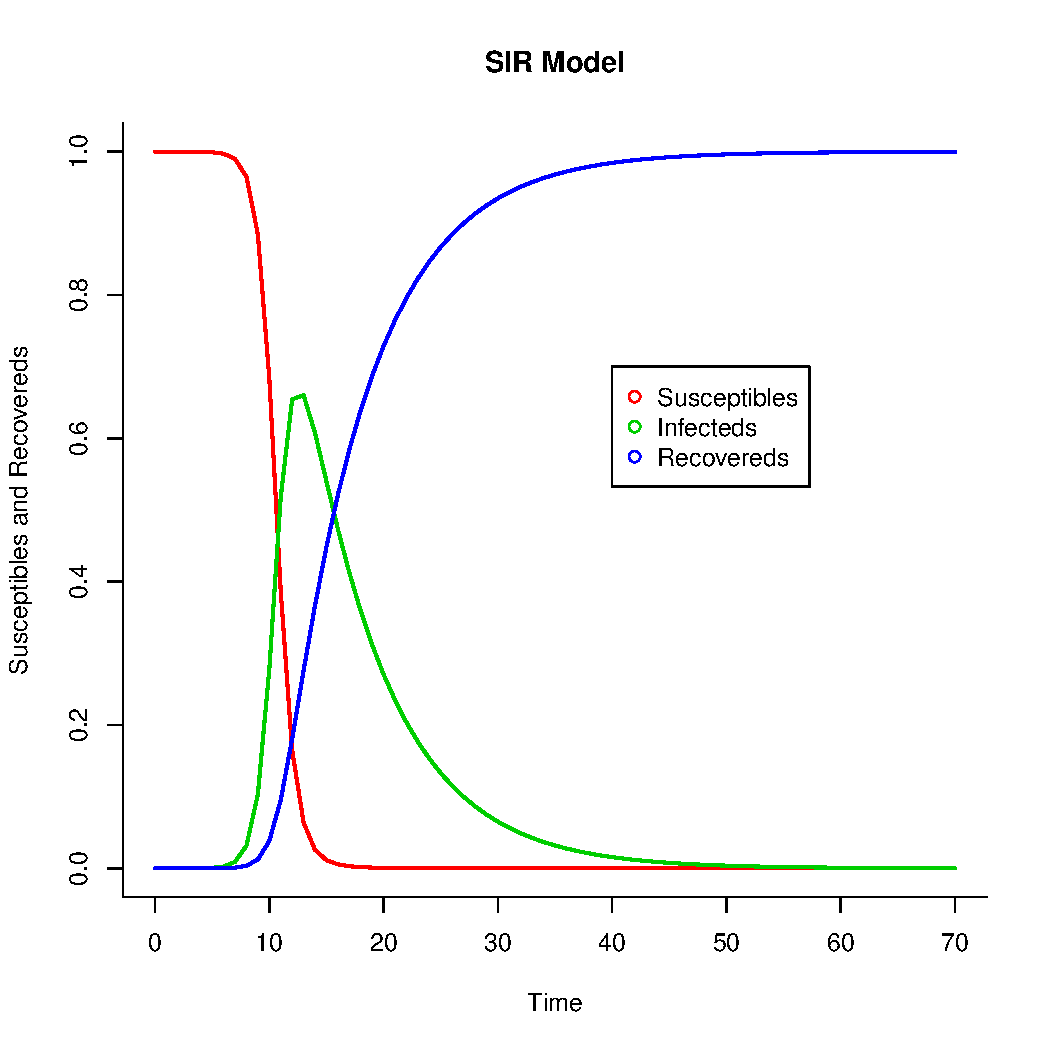
\includegraphics[width=\maxwidth]{figure/unnamed-chunk-2-1} 

\end{knitrout}


\subsection{Modeling Disease -- SEIR}

The first model is the basic SEIR without social distancing, then we add social distancing to show how the potential effectiveness of these strategies.

An extension of the classic SIR model and simply adds one more equation to show those who are exposed,

\begin{equation}\label{eq:dS2}
\dv{S}{t}	=	-\beta
\end{equation}

\begin{equation}\label{eq:dE2}
\dv{E}{t}	=	\beta SI - \omega E
\end{equation}

\begin{equation}\label{eq:dI2}
\dv{I}{t}	=	\omega E/N - \gamma I
\end{equation}


Equation \ref{eq:dS} is the change in people susceptible to the disease and is moderated by the number of infected people and their contact with the infected. Equation \ref{eq:dE} gives the people who have been exposed to the disease. It grows based on the contact rate and decreases based on the incubation period whereby people then become infected.

\subsection{SEIR with R}

In the case of $\beta$ is defined as $\beta_0$k, where $\beta_0$ is the probability of infection er expoure and k is the frequency of exposure. $\omega$ is the coeffecient of migration of latency and is estimated as $1/T_e$, where $T_e$ is the average latency. Finally, $\gamma$, which is $1/T_i$ is the recovery rate.

\begin{table}
\begin{tabular}{ll}\hline
Parameter     &  Model 1 \\  \hline\hline
$\beta_0$     & 0.1     \\
$k$           & 10      \\
$T_e$         & 7       \\
$T_i$         & 10.25 \\
\hline
\end{tabular}
\end{table}


\begin{knitrout}
\definecolor{shadecolor}{rgb}{0.969, 0.969, 0.969}\color{fgcolor}\begin{kframe}
\begin{alltt}
\hlstd{SEIR} \hlkwb{<-} \hlkwa{function}\hlstd{(}\hlkwc{beta0}\hlstd{,} \hlkwc{k}\hlstd{,} \hlkwc{Te}\hlstd{,} \hlkwc{Ti}\hlstd{)\{}

\hlcom{# Function to return derivatives of SEIR model}
\hlstd{seir_ode}\hlkwb{<-}\hlkwa{function}\hlstd{(}\hlkwc{t}\hlstd{,}\hlkwc{Y}\hlstd{,}\hlkwc{par}\hlstd{)\{}
  \hlstd{S}\hlkwb{<-}\hlstd{Y[}\hlnum{1}\hlstd{]}
  \hlstd{E}\hlkwb{<-}\hlstd{Y[}\hlnum{2}\hlstd{]}
  \hlstd{I}\hlkwb{<-}\hlstd{Y[}\hlnum{3}\hlstd{]}
  \hlstd{R}\hlkwb{<-}\hlstd{Y[}\hlnum{4}\hlstd{]}

  \hlstd{beta}\hlkwb{<-}\hlstd{par[}\hlnum{1}\hlstd{]}
  \hlstd{omega}\hlkwb{<-}\hlstd{par[}\hlnum{2}\hlstd{]}
  \hlstd{gamma}\hlkwb{<-}\hlstd{par[}\hlnum{3}\hlstd{]}
  \hlstd{mu}\hlkwb{<-}\hlstd{par[}\hlnum{4}\hlstd{]}

  \hlstd{dYdt}\hlkwb{<-}\hlkwd{vector}\hlstd{(}\hlkwc{length}\hlstd{=}\hlnum{3}\hlstd{)}
  \hlstd{dYdt[}\hlnum{1}\hlstd{]}\hlkwb{=}\hlstd{mu}\hlopt{-}\hlstd{beta}\hlopt{*}\hlstd{I}\hlopt{*}\hlstd{S}\hlopt{-}\hlstd{mu}\hlopt{*}\hlstd{S}
  \hlstd{dYdt[}\hlnum{2}\hlstd{]}\hlkwb{=}\hlstd{beta}\hlopt{*}\hlstd{I}\hlopt{*}\hlstd{S}\hlopt{-}\hlstd{(omega}\hlopt{+}\hlstd{mu)}\hlopt{*}\hlstd{E}
  \hlstd{dYdt[}\hlnum{3}\hlstd{]}\hlkwb{=}\hlstd{omega}\hlopt{*}\hlstd{E}\hlopt{-}\hlstd{(gamma}\hlopt{+}\hlstd{mu)}\hlopt{*}\hlstd{I}

  \hlkwd{return}\hlstd{(}\hlkwd{list}\hlstd{(dYdt))}
\hlstd{\}}
  \hlcom{# Set parameter values}
\hlstd{beta} \hlkwb{=} \hlstd{beta0}\hlopt{*}\hlstd{k}
\hlcom{#beta<-520/365;}
\hlstd{omega} \hlkwb{=} \hlnum{1}\hlopt{/}\hlstd{Te}
\hlcom{# sigma<-1/60;}
\hlstd{gamma} \hlkwb{=} \hlnum{1}\hlopt{/}\hlstd{Ti}
\hlcom{# gamma<-1/30;}
\hlstd{mu}\hlkwb{<-}\hlnum{774835}\hlopt{/}\hlstd{(}\hlnum{65640000}\hlopt{*}\hlnum{365}\hlstd{)} \hlcom{# UK birth and population figures 2016}
\hlcom{# mu=1000000}
\hlstd{init}\hlkwb{<-}\hlkwd{c}\hlstd{(}\hlnum{0.99}\hlstd{,}\hlnum{0.01}\hlstd{,}\hlnum{0.0}\hlstd{)}
\hlstd{t}\hlkwb{<-}\hlkwd{seq}\hlstd{(}\hlnum{0}\hlstd{,}\hlnum{365}\hlstd{)}
\hlstd{par}\hlkwb{<-}\hlkwd{c}\hlstd{(beta,omega,gamma,mu)}
\hlcom{# Solve system using lsoda}
\hlkwd{lsoda}\hlstd{(init,t,seir_ode,par)}
\hlstd{\}}

\hlstd{Model1} \hlkwb{<-} \hlkwd{SEIR}\hlstd{(}\hlnum{.1}\hlstd{,} \hlnum{10}\hlstd{,} \hlnum{7}\hlstd{,} \hlnum{10.25}\hlstd{)}
\end{alltt}
\end{kframe}
\end{knitrout}


\begin{knitrout}
\definecolor{shadecolor}{rgb}{0.969, 0.969, 0.969}\color{fgcolor}
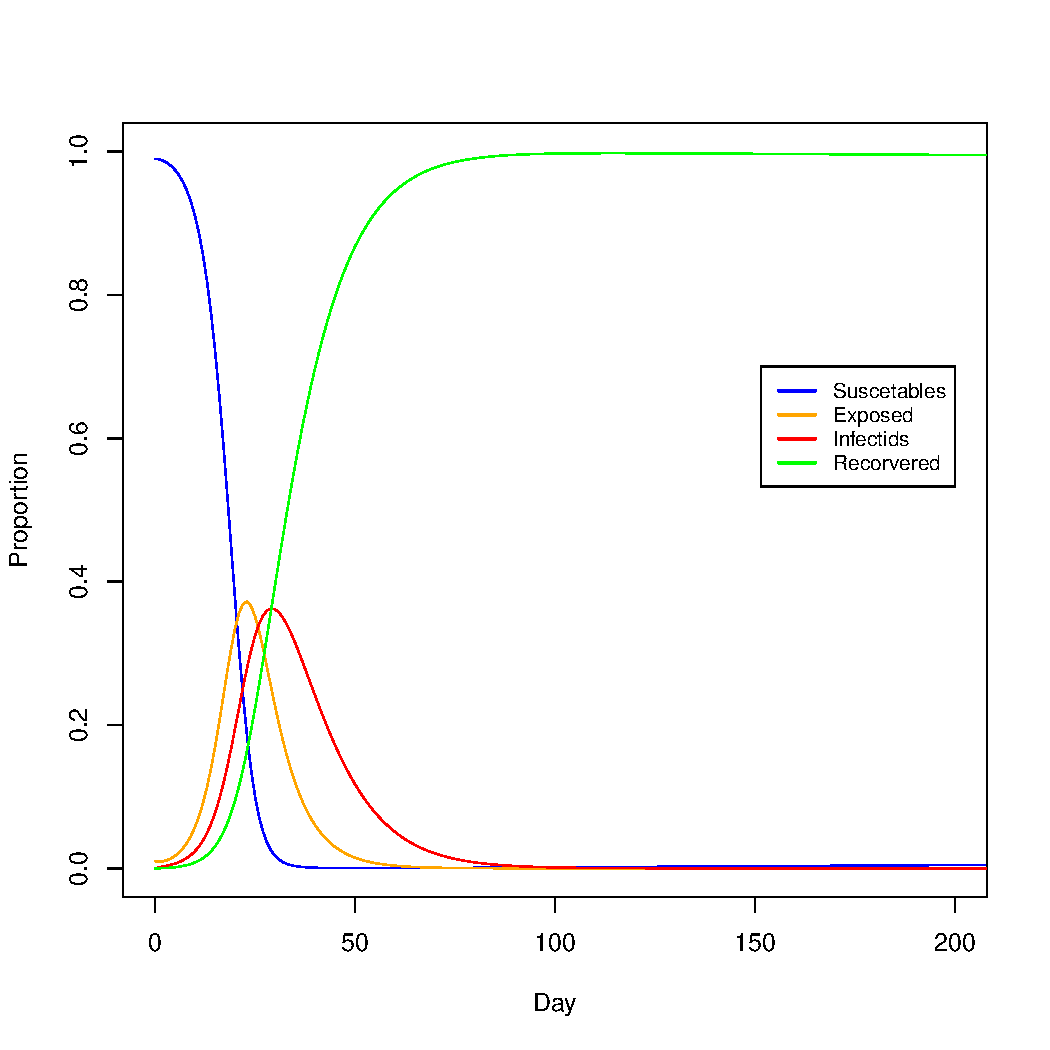
\includegraphics[width=\maxwidth]{figure/unnamed-chunk-4-1} 

\end{knitrout}


\subsection{SEIR-SEI and Disease Vectors}

When diseases are spread by vectors with their own dynamics, for example malaria and mosquitos, we should add additional compartments, namely suscecptability, exposure, and infection compartments for the mosquito. Mosquitos are not born with the malaria parasite, but must be infected from a host, so we can now include additional ODEs:

\begin{equation}\label{eq:dS3}
\dv{S_v}{t}	=	-\beta_v S_v I_v	/N
\end{equation}

\begin{equation}\label{eq:dI3}
\dv{I_v}{t}	=	\beta S_v I_v/N - \gamma I_v
\end{equation}

\begin{equation}\label{eq:dR3}
\dv{R_v}{t}	=	\gamma I_v,
\end{equation}

The key value governing the time evolution of these equations is the so-called epidemiological threshold and I think this can be used to link these two models, but I don't know how to yet.

\begin{equation}
 R_0= ?
\end{equation}

\begin{knitrout}
\definecolor{shadecolor}{rgb}{0.969, 0.969, 0.969}\color{fgcolor}\begin{kframe}
\begin{alltt}
\hlcom{# Function to return derivatives of SEIR model}
\hlstd{seir_ode}\hlkwb{<-}\hlkwa{function}\hlstd{(}\hlkwc{t}\hlstd{,}\hlkwc{Y}\hlstd{,}\hlkwc{par}\hlstd{)\{}
\hlcom{# Human Population}
  \hlstd{S}\hlkwb{<-}\hlstd{Y[}\hlnum{1}\hlstd{]}
  \hlstd{E}\hlkwb{<-}\hlstd{Y[}\hlnum{2}\hlstd{]}
  \hlstd{I}\hlkwb{<-}\hlstd{Y[}\hlnum{3}\hlstd{]}
  \hlstd{R}\hlkwb{<-}\hlstd{Y[}\hlnum{4}\hlstd{]}

  \hlstd{beta}\hlkwb{<-}\hlstd{par[}\hlnum{1}\hlstd{]}
  \hlstd{sigma}\hlkwb{<-}\hlstd{par[}\hlnum{2}\hlstd{]}
  \hlstd{gamma}\hlkwb{<-}\hlstd{par[}\hlnum{3}\hlstd{]}
  \hlstd{mu}\hlkwb{<-}\hlstd{par[}\hlnum{4}\hlstd{]}

  \hlstd{dYdt}\hlkwb{<-}\hlkwd{vector}\hlstd{(}\hlkwc{length}\hlstd{=}\hlnum{3}\hlstd{)}
  \hlstd{dYdt[}\hlnum{1}\hlstd{]}\hlkwb{=}\hlstd{mu}\hlopt{-}\hlstd{beta}\hlopt{*}\hlstd{I}\hlopt{*}\hlstd{S}\hlopt{-}\hlstd{mu}\hlopt{*}\hlstd{S}
  \hlstd{dYdt[}\hlnum{2}\hlstd{]}\hlkwb{=}\hlstd{beta}\hlopt{*}\hlstd{I}\hlopt{*}\hlstd{S}\hlopt{-}\hlstd{(sigma}\hlopt{+}\hlstd{mu)}\hlopt{*}\hlstd{E}
  \hlstd{dYdt[}\hlnum{3}\hlstd{]}\hlkwb{=}\hlstd{sigma}\hlopt{*}\hlstd{E}\hlopt{-}\hlstd{(gamma}\hlopt{+}\hlstd{mu)}\hlopt{*}\hlstd{I}

  \hlkwd{return}\hlstd{(}\hlkwd{list}\hlstd{(dYdt))}
\hlstd{\}}


\hlcom{# Set parameter values}
\hlstd{beta}\hlkwb{<-}\hlnum{520}\hlopt{/}\hlnum{365}\hlstd{;}
\hlstd{sigma}\hlkwb{<-}\hlnum{1}\hlopt{/}\hlnum{60}\hlstd{;}
\hlstd{gamma}\hlkwb{<-}\hlnum{1}\hlopt{/}\hlnum{30}\hlstd{;}
\hlstd{mu}\hlkwb{<-}\hlnum{774835}\hlopt{/}\hlstd{(}\hlnum{65640000}\hlopt{*}\hlnum{365}\hlstd{)} \hlcom{# UK birth and population figures 2016}
\hlstd{init}\hlkwb{<-}\hlkwd{c}\hlstd{(}\hlnum{0.8}\hlstd{,}\hlnum{0.1}\hlstd{,}\hlnum{0.1}\hlstd{)}
\hlstd{t}\hlkwb{<-}\hlkwd{seq}\hlstd{(}\hlnum{0}\hlstd{,}\hlnum{365}\hlstd{)}
\hlstd{par}\hlkwb{<-}\hlkwd{c}\hlstd{(beta,sigma,gamma,mu)}
\hlcom{# Solve system using lsoda}
\hlstd{sol}\hlkwb{<-}\hlkwd{lsoda}\hlstd{(init,t,seir_ode,par)}

\hlcom{# Plot solution}
\hlkwd{plot}\hlstd{(t,sol[,}\hlnum{2}\hlstd{],}\hlkwc{type}\hlstd{=}\hlstr{"l"}\hlstd{,}\hlkwc{col}\hlstd{=}\hlstr{"blue"}\hlstd{,}\hlkwc{ylim}\hlstd{=}\hlkwd{c}\hlstd{(}\hlnum{0}\hlstd{,}\hlnum{1}\hlstd{),}\hlkwc{ylab}\hlstd{=}\hlstr{"Proportion"}\hlstd{)}
\hlkwd{lines}\hlstd{(t,sol[,}\hlnum{3}\hlstd{],}\hlkwc{col}\hlstd{=}\hlstr{"orange"}\hlstd{)}
\hlkwd{lines}\hlstd{(t,sol[,}\hlnum{4}\hlstd{],}\hlkwc{col}\hlstd{=}\hlstr{"red"}\hlstd{)}
\hlkwd{lines}\hlstd{(t,}\hlnum{1}\hlopt{-}\hlkwd{rowSums}\hlstd{(sol[,}\hlnum{2}\hlopt{:}\hlnum{4}\hlstd{]),}\hlkwc{col}\hlstd{=}\hlstr{"green"}\hlstd{)}
\hlkwd{legend}\hlstd{(}\hlnum{300}\hlstd{,}\hlnum{0.7}\hlstd{,}\hlkwc{legend}\hlstd{=}\hlkwd{c}\hlstd{(}\hlstr{"S"}\hlstd{,}\hlstr{"E"}\hlstd{,}\hlstr{"I"}\hlstd{,}\hlstr{"R"}\hlstd{),}\hlkwc{col}\hlstd{=}\hlkwd{c}\hlstd{(}\hlstr{"blue"}\hlstd{,}\hlstr{"orange"}\hlstd{,}\hlstr{"red"}\hlstd{,}\hlstr{"green"}\hlstd{),} \hlkwc{lty}\hlstd{=}\hlnum{1}\hlstd{,} \hlkwc{cex}\hlstd{=}\hlnum{0.8}\hlstd{)}
\end{alltt}
\end{kframe}
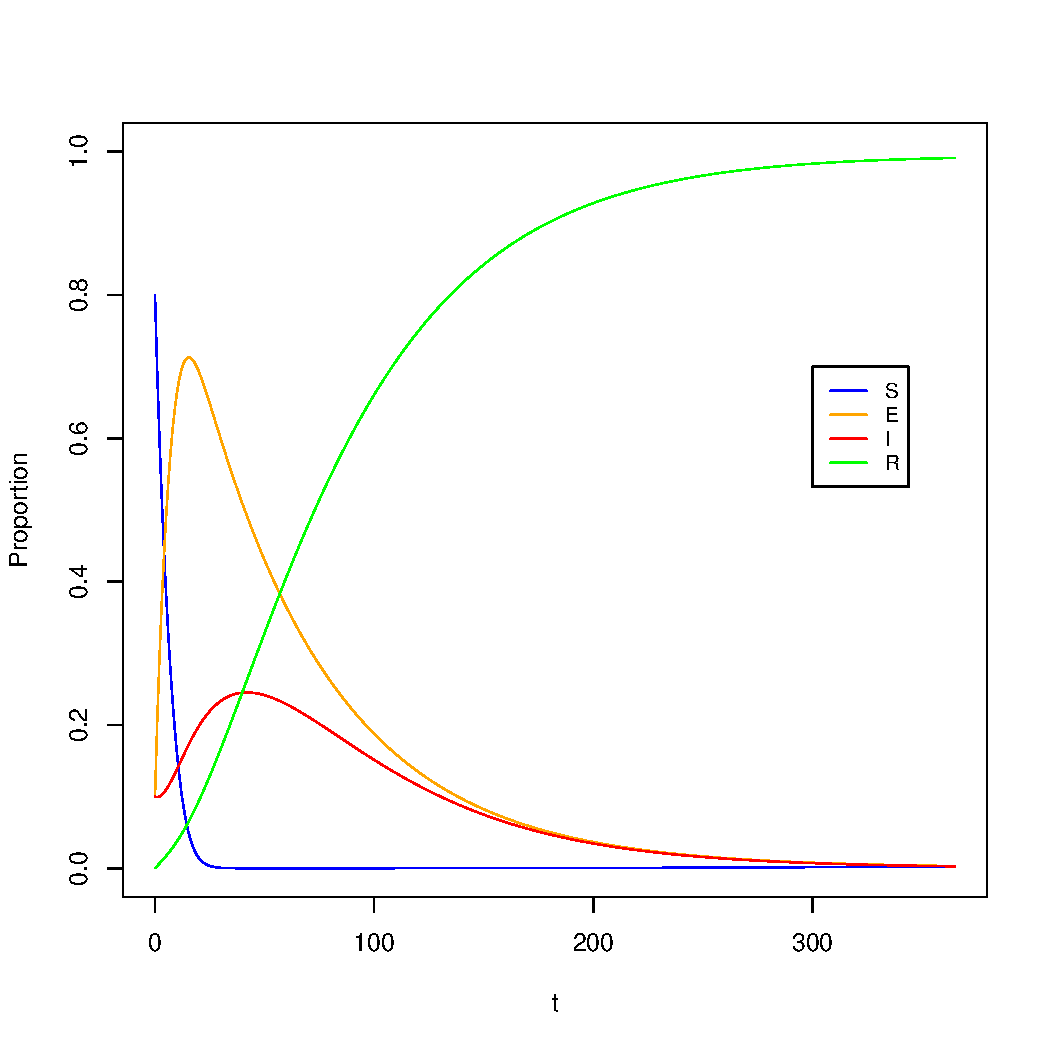
\includegraphics[width=\maxwidth]{figure/unnamed-chunk-5-1} 

\end{knitrout}


\section{Model with Spatial Structure}

\subsection{Model Structure}

The model relies on spatially explicit movements of 'subjects' that basically bounce around in a box, i.e. petri dish. Each subject is assigned a random location and trajectory (angle) of movement and velocity of movement vector. I based the model on an Washington Post article by Harry Stevens (March 14, 2020). Although his model, written in Java and is probably much cleaner, I wanted to create something that students could use to adjust parameters and evaluate different policy strategies, using a simple visualization as a foundation. 


\subsection{Building a Model}

To track subject movements, contact with others, etc I have defined an array to track subject, thus, have to do some backflips to track overlap at each time step to see if people are sharing space and pathogens. 

I'm not a programmer, so this is going to need some TLC as it's pretty ineffecient. 

\subsection{Model Parameterization}



I have define the following parameters for the model, which will be further described in each section below.

% latex table generated in R 3.6.0 by xtable 1.8-4 package
% Thu Apr  2 18:11:02 2020
\begin{table}[ht]
\centering
\begin{tabular}{rlrrrrrrrrr}
  \hline
 & Model & N & Velocity & tstep & Stationary & Inf\_Dist & init\_infact & asymp & symp & rec \\ 
  \hline
1 & Model1 & 50.00 & 5.00 & 2000.00 & 0.00 & 5.00 & 2.00 & 24.00 & 96.00 & 720.00 \\ 
  2 & Model2 & 100.00 & 5.00 & 2000.00 & 0.00 & 5.00 & 2.00 & 24.00 & 96.00 & 720.00 \\ 
  3 & Model3 & 100.00 & 5.00 & 3000.00 & 0.40 & 5.00 & 2.00 & 24.00 & 96.00 & 720.00 \\ 
  4 & Model4 & 100.00 & 5.00 & 3000.00 & 0.40 & 5.00 & 2.00 & 60.00 & 60.00 & 720.00 \\ 
  5 & TBD &  &  &  &  &  &  &  &  & 720.00 \\ 
  6 & Test & 5.00 & 5.00 & 20.00 & 0.00 & 300.00 & 1.00 & 24.00 & 96.00 & 720.00 \\ 
   \hline
\end{tabular}
\end{table}


But for now, I'd like to see how these align with the equations described above.

\subsection{Model Functions}

First, functions are useful when you have repetitive actions to make -- in this case, I have defined functions to move sujects based on their speed and direction of travel. 

Since these functions rely on the data array within another function (thus, not globally available, until it it `returned` at the end fo the function), I had to include a refernece to the data in the function so that the functions could find the array.

\begin{knitrout}
\definecolor{shadecolor}{rgb}{0.969, 0.969, 0.969}\color{fgcolor}\begin{kframe}
\begin{alltt}
\hlcom{#create function to move the subject}
\hlstd{move_x} \hlkwb{=} \hlkwa{function}\hlstd{(}\hlkwc{data_array}\hlstd{,} \hlkwc{s}\hlstd{,} \hlkwc{t}\hlstd{)\{}
\hlstd{data_array[s,} \hlnum{4}\hlstd{, t]} \hlopt{*} \hlkwd{cos}\hlstd{(data_array[s,}\hlnum{3}\hlstd{, t]}\hlopt{*}\hlstd{pi}\hlopt{/}\hlnum{180}\hlstd{)\}}
\hlstd{move_y} \hlkwb{=} \hlkwa{function}\hlstd{(}\hlkwc{data_array}\hlstd{,} \hlkwc{s}\hlstd{,} \hlkwc{t}\hlstd{)\{}
\hlstd{data_array[s,} \hlnum{4}\hlstd{, t]} \hlopt{*} \hlkwd{sin}\hlstd{(data_array[s,}\hlnum{3}\hlstd{, t]}\hlopt{*}\hlstd{pi}\hlopt{/}\hlnum{180}\hlstd{)\}}

\hlcom{# check function }
\hlcom{# move_y(data_arr, 1, 1); move_x(data_arr, 1,1)}

\hlcom{# move function}
\hlstd{move} \hlkwb{=} \hlkwa{function}\hlstd{(}\hlkwc{data_array}\hlstd{,} \hlkwc{s}\hlstd{,} \hlkwc{t}\hlstd{)\{}
  \hlkwd{c}\hlstd{(data_array[s,} \hlnum{1}\hlstd{, t}\hlopt{-}\hlnum{1}\hlstd{]}\hlopt{+} \hlkwd{move_x}\hlstd{(data_array, s, t}\hlopt{-}\hlnum{1}\hlstd{),}
    \hlstd{data_array[s,} \hlnum{2}\hlstd{, t}\hlopt{-}\hlnum{1}\hlstd{]}\hlopt{+} \hlkwd{move_y}\hlstd{(data_array, s, t}\hlopt{-}\hlnum{1}\hlstd{),}
    \hlstd{data_array[s,} \hlnum{3}\hlstd{, t}\hlopt{-}\hlnum{1}\hlstd{],}
    \hlstd{data_array[s,} \hlnum{4}\hlstd{, t}\hlopt{-}\hlnum{1}\hlstd{],}
    \hlstd{data_array[s,} \hlnum{5}\hlstd{, t}\hlopt{-}\hlnum{1}\hlstd{],}
    \hlstd{data_array[s,} \hlnum{6}\hlstd{, t}\hlopt{-}\hlnum{1}\hlstd{])}
\hlstd{\}}

\hlcom{# Test functions}
\hlcom{# data_arr[1,,1]}
\hlcom{# move(data_arr, 1, 2)}
\hlcom{# Model1; i = 2}
\end{alltt}
\end{kframe}
\end{knitrout}

\begin{knitrout}
\definecolor{shadecolor}{rgb}{0.969, 0.969, 0.969}\color{fgcolor}\begin{kframe}
\begin{alltt}
\hlcom{# Contact Infection Function}
\hlstd{contact} \hlkwb{=} \hlkwa{function}\hlstd{(}\hlkwc{data_array}\hlstd{,} \hlkwc{t}\hlstd{,} \hlkwc{Infect_dist}\hlstd{)\{}

\hlcom{# testfunction}
  \hlcom{#data_array=Model1_50; t=88; infect_dist = 5}
  \hlstd{pairs} \hlkwb{=} \hlkwd{cbind}\hlstd{(}\hlkwd{as.vector}\hlstd{(data_array[,}\hlstr{"x"}\hlstd{,t]),}
          \hlkwd{as.vector}\hlstd{(data_array[,}\hlstr{"y"}\hlstd{,t])); pairs}
  \hlstd{tmp} \hlkwb{=} \hlkwd{as.matrix}\hlstd{(}\hlkwd{dist}\hlstd{(pairs,} \hlkwc{method} \hlstd{=} \hlstr{"euclidean"} \hlstd{)); tmp}
  \hlstd{tmp[}\hlkwd{upper.tri}\hlstd{(tmp,} \hlkwc{diag} \hlstd{=} \hlnum{TRUE}\hlstd{)]} \hlkwb{<-} \hlnum{NA}\hlstd{; tmp}
  \hlstd{pairs} \hlkwb{<-} \hlkwd{which}\hlstd{(tmp} \hlopt{<} \hlstd{Infect_dist ,}\hlkwc{arr.ind} \hlstd{=} \hlnum{TRUE}\hlstd{);pairs}
  \hlstd{tmp2} \hlkwb{=} \hlkwd{cbind}\hlstd{(}\hlkwd{as.numeric}\hlstd{(}\hlkwd{rownames}\hlstd{(tmp)[pairs[,} \hlnum{1}\hlstd{]]),}
               \hlkwd{as.numeric}\hlstd{(}\hlkwd{colnames}\hlstd{(tmp)[pairs[,} \hlnum{2}\hlstd{]])); tmp2}
  \hlstd{contacts} \hlkwb{=} \hlkwd{dim}\hlstd{(tmp2)[}\hlnum{1}\hlstd{]; contacts}
  \hlkwa{if}\hlstd{(contacts}\hlopt{>}\hlnum{0}\hlstd{)\{}
    \hlkwa{for}\hlstd{(i} \hlkwa{in} \hlnum{1}\hlopt{:}\hlstd{contacts)\{}
      \hlcom{# If one is exposed, susceptable is exposed}
      \hlkwa{if}\hlstd{(data_array[tmp2[i,}\hlnum{1}\hlstd{],}\hlnum{5}\hlstd{,t]}\hlopt{==}\hlnum{2} \hlopt{&} \hlstd{data_array[tmp2[i,}\hlnum{2}\hlstd{],}\hlnum{5}\hlstd{,t]}\hlopt{==}\hlnum{1}\hlstd{)\{}
      \hlstd{data_array[tmp2[i,}\hlnum{2}\hlstd{],}\hlnum{5}\hlstd{,t]} \hlkwb{=} \hlnum{2}
      \hlstd{\}}
      \hlcom{# If one is exposed, susceptable is exposed}
      \hlkwa{if}\hlstd{(data_array[tmp2[i,}\hlnum{2}\hlstd{],}\hlnum{5}\hlstd{,t]}\hlopt{==}\hlnum{2} \hlopt{&} \hlstd{data_array[tmp2[i,}\hlnum{1}\hlstd{],}\hlnum{5}\hlstd{,t]}\hlopt{==}\hlnum{1}\hlstd{)\{}
      \hlstd{data_array[tmp2[i,}\hlnum{1}\hlstd{],}\hlnum{5}\hlstd{,t]} \hlkwb{=} \hlnum{2}
      \hlstd{\}}
      \hlcom{# If one is symptomatic, the susceptable is exposed}
      \hlkwa{if}\hlstd{(data_array[tmp2[i,}\hlnum{1}\hlstd{],}\hlnum{5}\hlstd{,t]}\hlopt{==}\hlnum{3} \hlopt{&} \hlstd{data_array[tmp2[i,}\hlnum{2}\hlstd{],}\hlnum{5}\hlstd{,t]}\hlopt{==}\hlnum{1}\hlstd{)\{}
      \hlstd{data_array[tmp2[i,}\hlnum{2}\hlstd{],} \hlnum{5}\hlstd{, t]} \hlkwb{=} \hlnum{2}
      \hlstd{\}}
      \hlcom{# If one is symptomatic, the susceptable is exposed}
      \hlkwa{if}\hlstd{(data_array[tmp2[i,}\hlnum{1}\hlstd{],}\hlnum{5}\hlstd{,t]}\hlopt{==}\hlnum{1} \hlopt{&} \hlstd{data_array[tmp2[i,}\hlnum{2}\hlstd{],}\hlnum{5}\hlstd{,t]}\hlopt{==}\hlnum{3}\hlstd{)\{}
      \hlstd{data_array[tmp2[i,}\hlnum{1}\hlstd{],} \hlnum{5}\hlstd{, t]} \hlkwb{=} \hlnum{2}
      \hlstd{\}}
    \hlstd{\}}

  \hlstd{\}}
   \hlcom{# data_array[,,t]}
\hlkwd{return}\hlstd{(data_array)}
\hlcom{# print(data_array[,5,t])}
\hlstd{\}} \hlcom{# close function}

\hlcom{#contact(Model1, 87, 5)}
\end{alltt}
\end{kframe}
\end{knitrout}

Next, I'm going to figure out how to create a function to text for euclidian distances to spread disease, but this will take some more effort \ldots

\subsection{Model 1: Modeling Susceptability and Infections  with No Behavior Changes and Recovery}

For this model, people get instantenously sick and start spreading it around -- not very realistic because when people get sick they are usually quarantined and stop bouncing around the environment. Nevertheless this sets up a good base line, where the poputation gets ill pretty quickly. 
\begin{knitrout}
\definecolor{shadecolor}{rgb}{0.969, 0.969, 0.969}\color{fgcolor}\begin{kframe}
\begin{alltt}
\hlstd{MoveSubjects} \hlkwb{=} \hlkwa{function}\hlstd{(}\hlkwc{m}\hlstd{=}\hlnum{0}\hlstd{)\{}
\hlcom{# m = 0}
\hlstd{N} \hlkwb{=} \hlstd{params[m,} \hlnum{2}\hlstd{]}
\hlstd{Velocity} \hlkwb{=} \hlstd{params[m,} \hlnum{3}\hlstd{]}
\hlstd{tstep} \hlkwb{=} \hlstd{params[m,} \hlnum{4}\hlstd{]}
\hlstd{Stationary} \hlkwb{=} \hlstd{params[m,}\hlnum{5}\hlstd{];}
\hlstd{Infect_dist}\hlkwb{=}\hlstd{params[m,} \hlnum{6}\hlstd{];}
\hlstd{Init_infect}\hlkwb{=}\hlstd{params[m,} \hlnum{7}\hlstd{]}
\hlstd{asymp} \hlkwb{=} \hlstd{params[m,}\hlnum{8}\hlstd{]}
\hlstd{symp} \hlkwb{=} \hlstd{params[m,}\hlnum{9}\hlstd{]}
\hlstd{rec} \hlkwb{=} \hlstd{params[m,}\hlnum{10}\hlstd{]}

\hlcom{# Define Data Array}
\hlstd{location} \hlkwb{=} \hlnum{6} \hlcom{# number of parameters to track}
\hlstd{data_arr} \hlkwb{=} \hlkwd{array}\hlstd{(}\hlkwc{dim}\hlstd{=}\hlkwd{c}\hlstd{(N, location, tstep))}
\hlkwd{dimnames}\hlstd{(data_arr)[[}\hlnum{2}\hlstd{]]} \hlkwb{<-} \hlkwd{c}\hlstd{(}\hlstr{"x"}\hlstd{,} \hlstr{"y"}\hlstd{,} \hlstr{"theta"}\hlstd{,} \hlstr{"velocity"}\hlstd{,} \hlstr{"status"}\hlstd{,} \hlstr{"count"}\hlstd{)}
\hlstd{data_arr[,,}\hlnum{1}\hlstd{]}
\hlcom{# Initialize Start Locations}
\hlkwd{set.seed}\hlstd{(}\hlnum{2763}\hlstd{)}
\hlstd{subj_x} \hlkwb{=} \hlkwd{runif}\hlstd{(N, coord_range[}\hlnum{1}\hlstd{],  coord_range[}\hlnum{2}\hlstd{]); subj_x}
\hlstd{subj_y} \hlkwb{=} \hlkwd{runif}\hlstd{(N, coord_range[}\hlnum{3}\hlstd{],  coord_range[}\hlnum{4}\hlstd{]); subj_y}

\hlcom{# Set Up Population Characteristics and Behaviors}
\hlstd{sheltered} \hlkwb{=} \hlkwd{sample}\hlstd{(N}\hlopt{*}\hlstd{Stationary); sheltered}
\hlstd{velocity} \hlkwb{=} \hlkwd{rep}\hlstd{(Velocity,N); velocity[sheltered]}\hlkwb{=}\hlnum{0}\hlstd{; velocity}
\hlstd{theta} \hlkwb{=} \hlkwd{round}\hlstd{(}\hlkwd{runif}\hlstd{(N,} \hlnum{0}\hlstd{,} \hlnum{360}\hlstd{),}\hlnum{0}\hlstd{); theta}
\hlstd{SEIR} \hlkwb{=} \hlkwd{rep}\hlstd{(}\hlnum{1}\hlstd{, N); SEIR[sheltered]} \hlkwb{=} \hlnum{0}
\hlstd{SEIR[}\hlkwd{sample}\hlstd{(N, Init_infect)]} \hlkwb{=} \hlnum{3}\hlstd{; SEIR}
\hlstd{count} \hlkwb{=} \hlkwd{rep}\hlstd{(}\hlnum{0}\hlstd{, N)}

\hlcom{# Initial Locations}
\hlstd{data_arr[,,}\hlnum{1}\hlstd{]} \hlkwb{=} \hlkwd{c}\hlstd{(subj_x, subj_y, theta, velocity, SEIR, count)}
\hlstd{data_arr[,,}\hlnum{1}\hlstd{]}
\hlcom{# t = 2; s=1}
\hlkwa{for}\hlstd{(t} \hlkwa{in} \hlnum{2}\hlopt{:}\hlstd{tstep)\{}
  \hlkwa{for}\hlstd{(s} \hlkwa{in} \hlnum{1}\hlopt{:}\hlstd{N)\{}
    \hlcom{# move subjects based on theta and speed}
    \hlstd{data_arr[s,,t]} \hlkwb{=} \hlkwd{move}\hlstd{(data_arr, s, t)}
    \hlcom{# coarse corrections when hitting a boundary}
    \hlcom{# Min x-boundary}
    \hlkwa{if}\hlstd{(data_arr[s,}\hlnum{1}\hlstd{,t]} \hlopt{<} \hlstd{coord_range[}\hlnum{1}\hlstd{])\{}
      \hlstd{data_arr[s,}\hlnum{3}\hlstd{,t}\hlopt{-}\hlnum{1}\hlstd{]}\hlkwb{=}\hlnum{180}\hlopt{-}\hlstd{data_arr[s,}\hlnum{3}\hlstd{,t}\hlopt{-}\hlnum{1}\hlstd{]}
      \hlstd{data_arr[s,,t]} \hlkwb{=} \hlkwd{move}\hlstd{(data_arr, s, t)}
    \hlstd{\}}
    \hlcom{#Max x-boundary}
    \hlkwa{if}\hlstd{(data_arr[s,}\hlnum{1}\hlstd{,t]} \hlopt{>} \hlstd{coord_range[}\hlnum{2}\hlstd{])\{}
      \hlstd{data_arr[s,}\hlnum{3}\hlstd{,t}\hlopt{-}\hlnum{1}\hlstd{]}\hlkwb{=}\hlnum{180}\hlopt{-}\hlstd{data_arr[s,}\hlnum{3}\hlstd{,t}\hlopt{-}\hlnum{1}\hlstd{]}
      \hlstd{data_arr[s,,t]} \hlkwb{=} \hlkwd{move}\hlstd{(data_arr, s, t)}
    \hlstd{\}}
    \hlcom{#Min y-boundary}
    \hlkwa{if}\hlstd{(data_arr[s,}\hlnum{2}\hlstd{,t]} \hlopt{<} \hlstd{coord_range[}\hlnum{3}\hlstd{])\{}
      \hlstd{data_arr[s,}\hlnum{3}\hlstd{,t}\hlopt{-}\hlnum{1}\hlstd{]}\hlkwb{=}\hlnum{360}\hlopt{-}\hlstd{data_arr[s,}\hlnum{3}\hlstd{,t}\hlopt{-}\hlnum{1}\hlstd{]}
      \hlstd{data_arr[s,,t]} \hlkwb{=} \hlkwd{move}\hlstd{(data_arr, s, t)}
    \hlstd{\}}
    \hlcom{#Max y-boundary}
    \hlkwa{if}\hlstd{(data_arr[s,}\hlnum{2}\hlstd{,t]} \hlopt{>} \hlstd{coord_range[}\hlnum{4}\hlstd{])\{}
      \hlstd{data_arr[s,}\hlnum{3}\hlstd{,t}\hlopt{-}\hlnum{1}\hlstd{]}\hlkwb{=}\hlnum{360}\hlopt{-}\hlstd{data_arr[s,}\hlnum{3}\hlstd{,t}\hlopt{-}\hlnum{1}\hlstd{]}
      \hlstd{data_arr[s,,t]} \hlkwb{=} \hlkwd{move}\hlstd{(data_arr, s, t)}
    \hlstd{\}}
    \hlcom{# Change Status based on Time Steps}
    \hlstd{data_arr[s,}\hlnum{6}\hlstd{,t]} \hlkwb{=} \hlstd{data_arr[s,}\hlnum{6}\hlstd{,t]} \hlopt{+} \hlnum{1}
    \hlkwa{if}\hlstd{(data_arr[s,}\hlnum{5}\hlstd{,t]}\hlopt{==}\hlnum{1} \hlopt{|} \hlstd{data_arr[s,}\hlnum{5}\hlstd{,t]}\hlopt{==}\hlnum{0}\hlstd{) data_arr[s,}\hlnum{6}\hlstd{,t]}\hlkwb{=}\hlnum{0} \hlcom{# Reset Susceptables  }
   \hlcom{# Exposed becomes symptomatic}
  \hlkwa{if}\hlstd{(data_arr[s,}\hlnum{5}\hlstd{,t]}\hlopt{==}\hlnum{2} \hlopt{&} \hlstd{data_arr[s,}\hlnum{6}\hlstd{,t]} \hlopt{>} \hlstd{asymp)\{}
    \hlstd{data_arr[s,}\hlnum{5}\hlstd{,t]}\hlkwb{=}\hlnum{3}\hlstd{\}}
    \hlcom{# Symptomatics move very little}
  \hlkwa{if}\hlstd{(data_arr[s,}\hlnum{5}\hlstd{,t]}\hlopt{==}\hlnum{3} \hlopt{&} \hlstd{data_arr[s,}\hlnum{6}\hlstd{,t]} \hlopt{>} \hlstd{symp)\{}
    \hlstd{data_arr[s,}\hlnum{4}\hlstd{,t]} \hlkwb{=} \hlstd{Velocity}\hlopt{/}\hlnum{2}\hlstd{\}}
  \hlcom{# Time to Recovery}
  \hlkwa{if}\hlstd{(data_arr[s,}\hlnum{5}\hlstd{,t]}\hlopt{==}\hlnum{3} \hlopt{&} \hlstd{data_arr[s,}\hlnum{6}\hlstd{,t]} \hlopt{>} \hlstd{rec)\{}
    \hlstd{data_arr[s,}\hlnum{5}\hlstd{,t]} \hlkwb{=} \hlnum{4}
    \hlstd{data_arr[s,}\hlnum{4}\hlstd{,t]} \hlkwb{=} \hlstd{Velocity}
    \hlstd{\}}
  \hlstd{\}} \hlcom{# End of Subj Moving}

  \hlcom{# Time Step Proceesing}
  \hlcom{# Test for Euclidean Distances Here!}

\hlstd{data_arr} \hlkwb{<-} \hlkwd{contact}\hlstd{(data_arr, t, Infect_dist)}

\hlstd{\}} \hlcom{# End of Time Step}
\hlkwd{return}\hlstd{(data_arr)}
\hlstd{\}}
\end{alltt}
\end{kframe}
\end{knitrout}

\subsection{Model Runs}

For after running the models, I visually evaluated the models to make sure there weren't unintended consequences, i.e. usually from coding errors. Below are the models that I ran and the estimated run times. 

\begin{knitrout}
\definecolor{shadecolor}{rgb}{0.969, 0.969, 0.969}\color{fgcolor}\begin{kframe}
\begin{alltt}
\hlkwd{library}\hlstd{(tictoc)}
\hlcom{#N=3, tstep=4, speed=5, init_infect=1, stationary = 0)}
\hlstd{params}

\hlkwd{tic}\hlstd{(}\hlstr{"Model0"}\hlstd{)}
\hlstd{Test}\hlkwb{<-} \hlkwd{MoveSubjects}\hlstd{(}\hlkwc{m}\hlstd{=}\hlnum{6}\hlstd{)}
\hlkwd{toc}\hlstd{()} \hlcom{# .02s}

\hlkwd{tic}\hlstd{(}\hlstr{"Model1"}\hlstd{)}
\hlstd{Model1}\hlkwb{<-} \hlkwd{MoveSubjects}\hlstd{(}\hlkwc{m}\hlstd{=}\hlnum{1}\hlstd{)}
\hlkwd{toc}\hlstd{()} \hlcom{# 900s; 314s}

\hlkwd{tic}\hlstd{(}\hlstr{"Model2"}\hlstd{)}
\hlstd{Model2}\hlkwb{<-} \hlkwd{MoveSubjects}\hlstd{(}\hlkwc{m}\hlstd{=}\hlnum{2}\hlstd{)}
\hlkwd{toc}\hlstd{()} \hlcom{#1800s; 1158s; 1313s}

\hlkwd{tic}\hlstd{(}\hlstr{"Model3"}\hlstd{)}
\hlstd{Model3} \hlkwb{<-} \hlkwd{MoveSubjects}\hlstd{(}\hlkwc{m}\hlstd{=}\hlnum{3}\hlstd{)}
\hlkwd{toc}\hlstd{()} \hlcom{#3308; 2437s; 2599s}

\hlkwd{tic}\hlstd{(}\hlstr{"Model4"}\hlstd{)}
\hlstd{Model4} \hlkwb{<-} \hlkwd{MoveSubjects}\hlstd{(}\hlkwc{m}\hlstd{=}\hlnum{4}\hlstd{)}
\hlkwd{toc}\hlstd{()} \hlcom{#3308s; 2332s; 2616s}
\end{alltt}
\end{kframe}
\end{knitrout}

\section{Visualizations}

\subsection{Tracking the Disease Transfer}

\begin{knitrout}
\definecolor{shadecolor}{rgb}{0.969, 0.969, 0.969}\color{fgcolor}\begin{kframe}
\begin{alltt}
\hlcom{#load("/home/CAMPUS/mwl04747/github/beginnersluck.RData")}
\hlcom{# Susceptable 1, Exposed-Asymptomatic 2, Symptomatic 3, Recovered 4}
\hlstd{SEIRcol} \hlkwb{=} \hlkwd{c}\hlstd{(}\hlstr{"steelblue"}\hlstd{,} \hlstr{"orange"}\hlstd{,}\hlstr{"red"}\hlstd{,} \hlstr{"green"}\hlstd{)}

\hlstd{trackresults}\hlkwb{=}\hlkwa{function}\hlstd{(}\hlkwc{model}\hlstd{,}\hlkwc{m}\hlstd{,}\hlkwc{tstep}\hlstd{)\{}
\hlstd{results} \hlkwb{=} \hlkwd{data.frame}\hlstd{(}\hlkwc{Days} \hlstd{=} \hlnum{NA}\hlstd{,} \hlkwc{Sh} \hlstd{=} \hlnum{NA}\hlstd{,} \hlkwc{S}\hlstd{=}\hlnum{NA}\hlstd{,} \hlkwc{E}\hlstd{=}\hlnum{NA}\hlstd{,} \hlkwc{I}\hlstd{=}\hlnum{NA}\hlstd{,} \hlkwc{R}\hlstd{=}\hlnum{NA}\hlstd{)}
\hlkwa{for}\hlstd{(t} \hlkwa{in} \hlnum{1}\hlopt{:}\hlstd{tstep)\{}
\hlstd{days} \hlkwb{=} \hlstd{t}\hlopt{/}\hlnum{24}
\hlstd{sh} \hlkwb{=} \hlkwd{sum}\hlstd{(}\hlkwd{as.vector}\hlstd{(model[,}\hlnum{5}\hlstd{,t])}\hlopt{==}\hlnum{0}\hlstd{)}
\hlstd{s} \hlkwb{=} \hlkwd{sum}\hlstd{(}\hlkwd{as.vector}\hlstd{(model[,}\hlnum{5}\hlstd{,t])}\hlopt{==}\hlnum{1}\hlstd{, sh)}
\hlstd{e} \hlkwb{=} \hlkwd{sum}\hlstd{(}\hlkwd{as.vector}\hlstd{(model[,}\hlnum{5}\hlstd{,t])}\hlopt{==}\hlnum{2}\hlstd{)}
\hlstd{i} \hlkwb{=} \hlkwd{sum}\hlstd{(}\hlkwd{as.vector}\hlstd{(model[,}\hlnum{5}\hlstd{,t])}\hlopt{==}\hlnum{3}\hlstd{)}
\hlstd{r} \hlkwb{=} \hlkwd{sum}\hlstd{(}\hlkwd{as.vector}\hlstd{(model[,}\hlnum{5}\hlstd{,t])}\hlopt{==}\hlnum{4}\hlstd{)}
\hlstd{results[t,]} \hlkwb{<-} \hlkwd{data.frame}\hlstd{(}\hlkwc{Days} \hlstd{= days,} \hlkwc{Sh} \hlstd{= sh,} \hlkwc{S}\hlstd{=s,} \hlkwc{E}\hlstd{=e,} \hlkwc{I}\hlstd{=i,} \hlkwc{R}\hlstd{=r)}
\hlstd{\}}
\hlkwd{head}\hlstd{(results)}
\hlkwd{par}\hlstd{(}\hlkwc{mfrow}\hlstd{=}\hlkwd{c}\hlstd{(}\hlnum{1}\hlstd{,}\hlnum{1}\hlstd{),} \hlkwc{mar}\hlstd{=}\hlkwd{c}\hlstd{(}\hlnum{4}\hlstd{,} \hlnum{5}\hlstd{,} \hlnum{3}\hlstd{,} \hlnum{2}\hlstd{)}\hlopt{+}\hlnum{.1}\hlstd{,} \hlkwc{las}\hlstd{=}\hlnum{1}\hlstd{)}
\hlkwd{plot}\hlstd{(S}\hlopt{~}\hlstd{Days,} \hlkwc{data}\hlstd{=results,} \hlkwc{ty}\hlstd{=}\hlstr{'l'}\hlstd{,} \hlkwc{col}\hlstd{=SEIRcol[}\hlnum{1}\hlstd{],} \hlkwc{ylab}\hlstd{=}\hlstr{""}\hlstd{,} \hlkwc{ylim}\hlstd{=}\hlkwd{c}\hlstd{(}\hlnum{0}\hlstd{,params[m,}\hlnum{2}\hlstd{]),} \hlkwc{xlab}\hlstd{=}\hlstr{"Days"}\hlstd{,} \hlkwc{xlim}\hlstd{=}\hlkwd{c}\hlstd{(}\hlnum{0}\hlstd{,tstep}\hlopt{/}\hlnum{24}\hlstd{),} \hlkwc{lwd}\hlstd{=}\hlnum{2}\hlstd{,} \hlkwc{main} \hlstd{=} \hlkwd{paste}\hlstd{(params[m,} \hlnum{1}\hlstd{],} \hlstr{", Stationary ="}\hlstd{, params[m,}\hlnum{5}\hlstd{]}\hlopt{*}\hlnum{100}\hlstd{,} \hlstr{"%"}\hlstd{))}
\hlkwd{lines}\hlstd{(E}\hlopt{~}\hlstd{Days,} \hlkwc{data}\hlstd{=results,} \hlkwc{col}\hlstd{=SEIRcol[}\hlnum{2}\hlstd{],} \hlkwc{lwd}\hlstd{=}\hlnum{2}\hlstd{)}
\hlkwd{lines}\hlstd{(I}\hlopt{~}\hlstd{Days,} \hlkwc{data}\hlstd{=results,} \hlkwc{col}\hlstd{=SEIRcol[}\hlnum{3}\hlstd{],} \hlkwc{lwd}\hlstd{=}\hlnum{2}\hlstd{)}
\hlkwd{lines}\hlstd{(R}\hlopt{~}\hlstd{Days,} \hlkwc{data}\hlstd{=results,} \hlkwc{col}\hlstd{=SEIRcol[}\hlnum{4}\hlstd{],} \hlkwc{lwd}\hlstd{=}\hlnum{2}\hlstd{)}
\hlstd{\}}

\hlstd{m} \hlkwb{=} \hlnum{6}\hlstd{;} \hlkwd{trackresults}\hlstd{(Test, m, params[m,}\hlnum{4}\hlstd{])}

\hlkwd{png}\hlstd{(}\hlkwc{filename} \hlstd{=}
  \hlstr{"/home/CAMPUS/mwl04747/github/beginnersluck/Epidemiology/Model1.png"}\hlstd{);}
  \hlstd{m} \hlkwb{=} \hlnum{1}\hlstd{;} \hlkwd{trackresults}\hlstd{(Model1, m,} \hlnum{2000}\hlstd{);} \hlkwd{dev.off}\hlstd{()}
\hlkwd{png}\hlstd{(}\hlkwc{filename} \hlstd{=}
  \hlstr{"/home/CAMPUS/mwl04747/github/beginnersluck/Epidemiology/Model2.png"}\hlstd{);}
  \hlstd{m} \hlkwb{=} \hlnum{2}\hlstd{;} \hlkwd{trackresults}\hlstd{(Model2, m,} \hlnum{2000}\hlstd{);} \hlkwd{dev.off}\hlstd{()}
\hlkwd{png}\hlstd{(}\hlkwc{filename} \hlstd{=}
  \hlstr{"/home/CAMPUS/mwl04747/github/beginnersluck/Epidemiology/Model3.png"}\hlstd{);}
  \hlstd{m} \hlkwb{=} \hlnum{3}\hlstd{;} \hlkwd{trackresults}\hlstd{(Model3, m,} \hlnum{2000}\hlstd{);} \hlkwd{dev.off}\hlstd{()}
\hlkwd{png}\hlstd{(}\hlkwc{filename} \hlstd{=}
  \hlstr{"/home/CAMPUS/mwl04747/github/beginnersluck/Epidemiology/Model4.png"}\hlstd{);}
  \hlstd{m} \hlkwb{=} \hlnum{4}\hlstd{;} \hlkwd{trackresults}\hlstd{(Model4, m,} \hlnum{2000}\hlstd{);} \hlkwd{dev.off}\hlstd{()}
\end{alltt}
\end{kframe}
\end{knitrout}

\begin{figure}
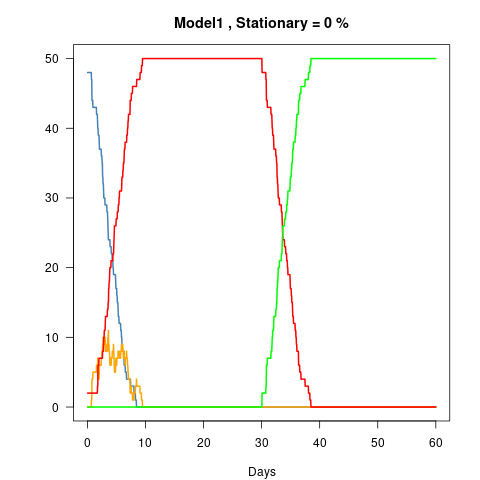
\includegraphics[width=1\textwidth]{Model1.png}
\caption{N = 50}
\end{figure}

\begin{figure}
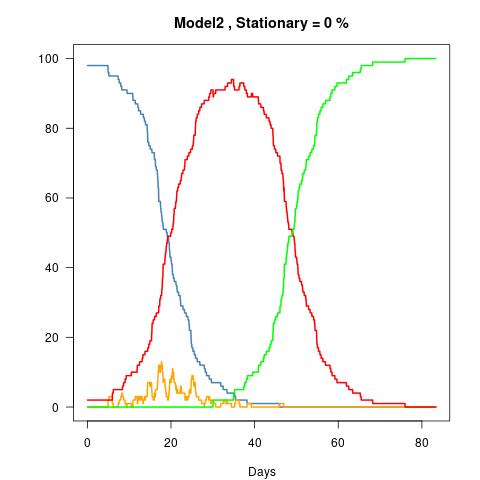
\includegraphics[width=1\textwidth]{Model2.png}
\caption{N=100}
\end{figure}

\begin{figure}
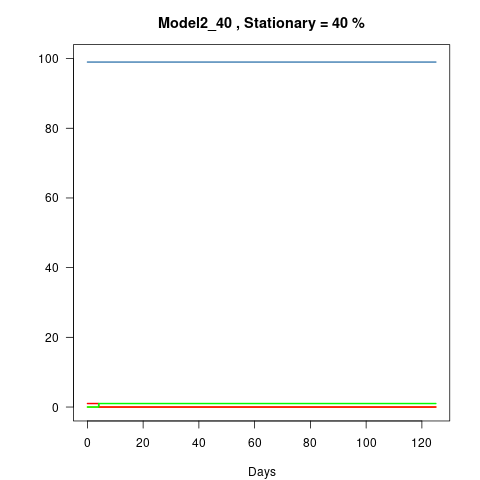
\includegraphics[width=1\textwidth]{Model3.png}
\caption{40\% shelter in place}
\end{figure}

\begin{figure}
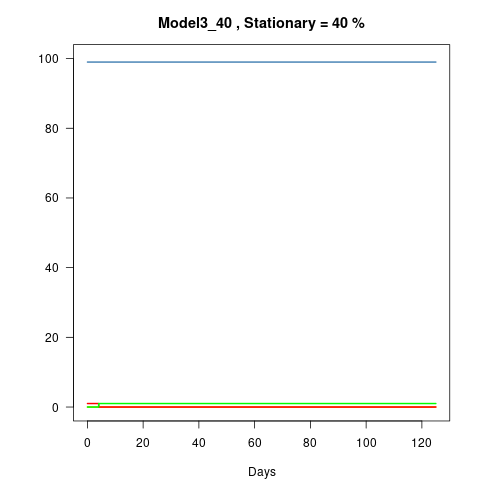
\includegraphics[width=1\textwidth]{Model4.png}
\caption{40\% shelter in place, exposed without symptoms.}
\end{figure}

\subsection{Static Spatial Plots}

Because we are looking at a dynamic system, I don't find the static plot all that useful.



\begin{figure}
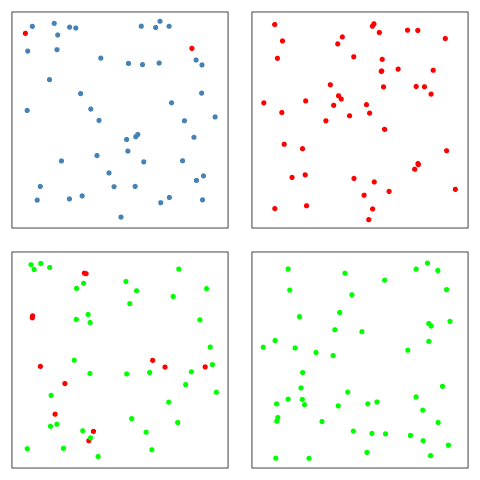
\includegraphics[width=1\textwidth]{SSModel1.png}
\caption{N = 50}
\end{figure}

\begin{figure}
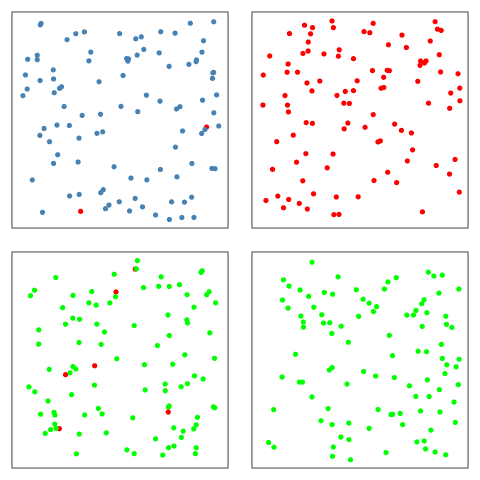
\includegraphics[width=1\textwidth]{SSModel2.png}
\caption{N=100}
\end{figure}

\begin{figure}
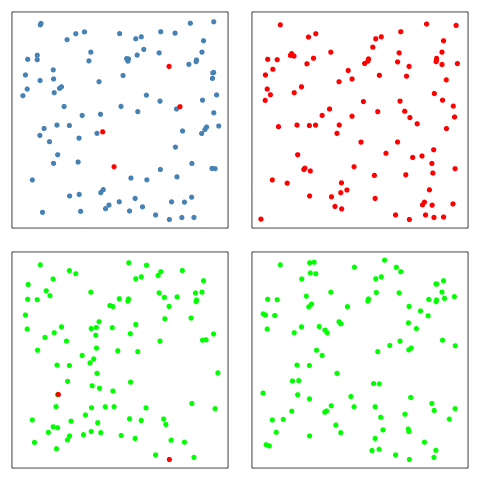
\includegraphics[width=1\textwidth]{SSModel3.png}
\caption{40\% shelter in place}
\end{figure}

\begin{figure}
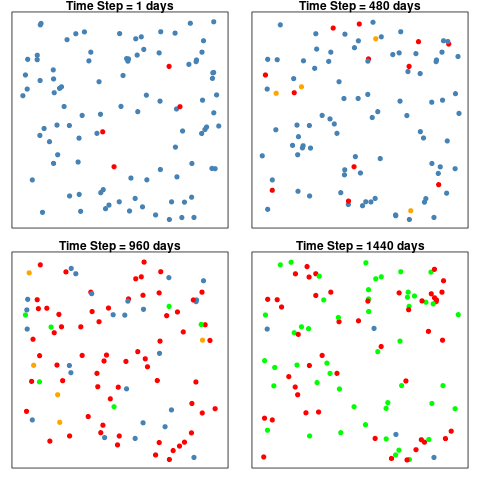
\includegraphics[width=1\textwidth]{SSModel4.png}
\caption{40\% shelter in place, exposed without symptoms.}
\end{figure}
\subsection{Animating the Results}

Still working on this... I have to export the file to my laptop then use photoshop to make a movie.

it would be nice to do this in r and then embedd in a pdf...




\section{SEIRS with vital dynamics}

You can also add vital dynamics to an SEIRS model, where $\mu$ and $\nu$ represent the birth and death rates, respectively. To maintain a constant population, assume that $\mu$ = $\nu$. In steady state $\frac{dI}{dt} = 0$. The ODE then becomes:

\begin{equation}
\dv{S}{t}  = \mu N - \frac{\beta S I}{N} + \xi R- \nu S
\end{equation}

\begin{equation}
\dv{E}{t}  = \frac{\beta S I}{N} - \sigma E - \nu E
\end{equation}

\begin{equation}
\dv{I}{t}  = \sigma E - \gamma I - \nu I\\
\end{equation}


\begin{equation}
\dv{R}{t}  = \gamma I - \xi R - \nu R
\end{equation}

where N = S + E + I + R is the total population.

\begin{figure}
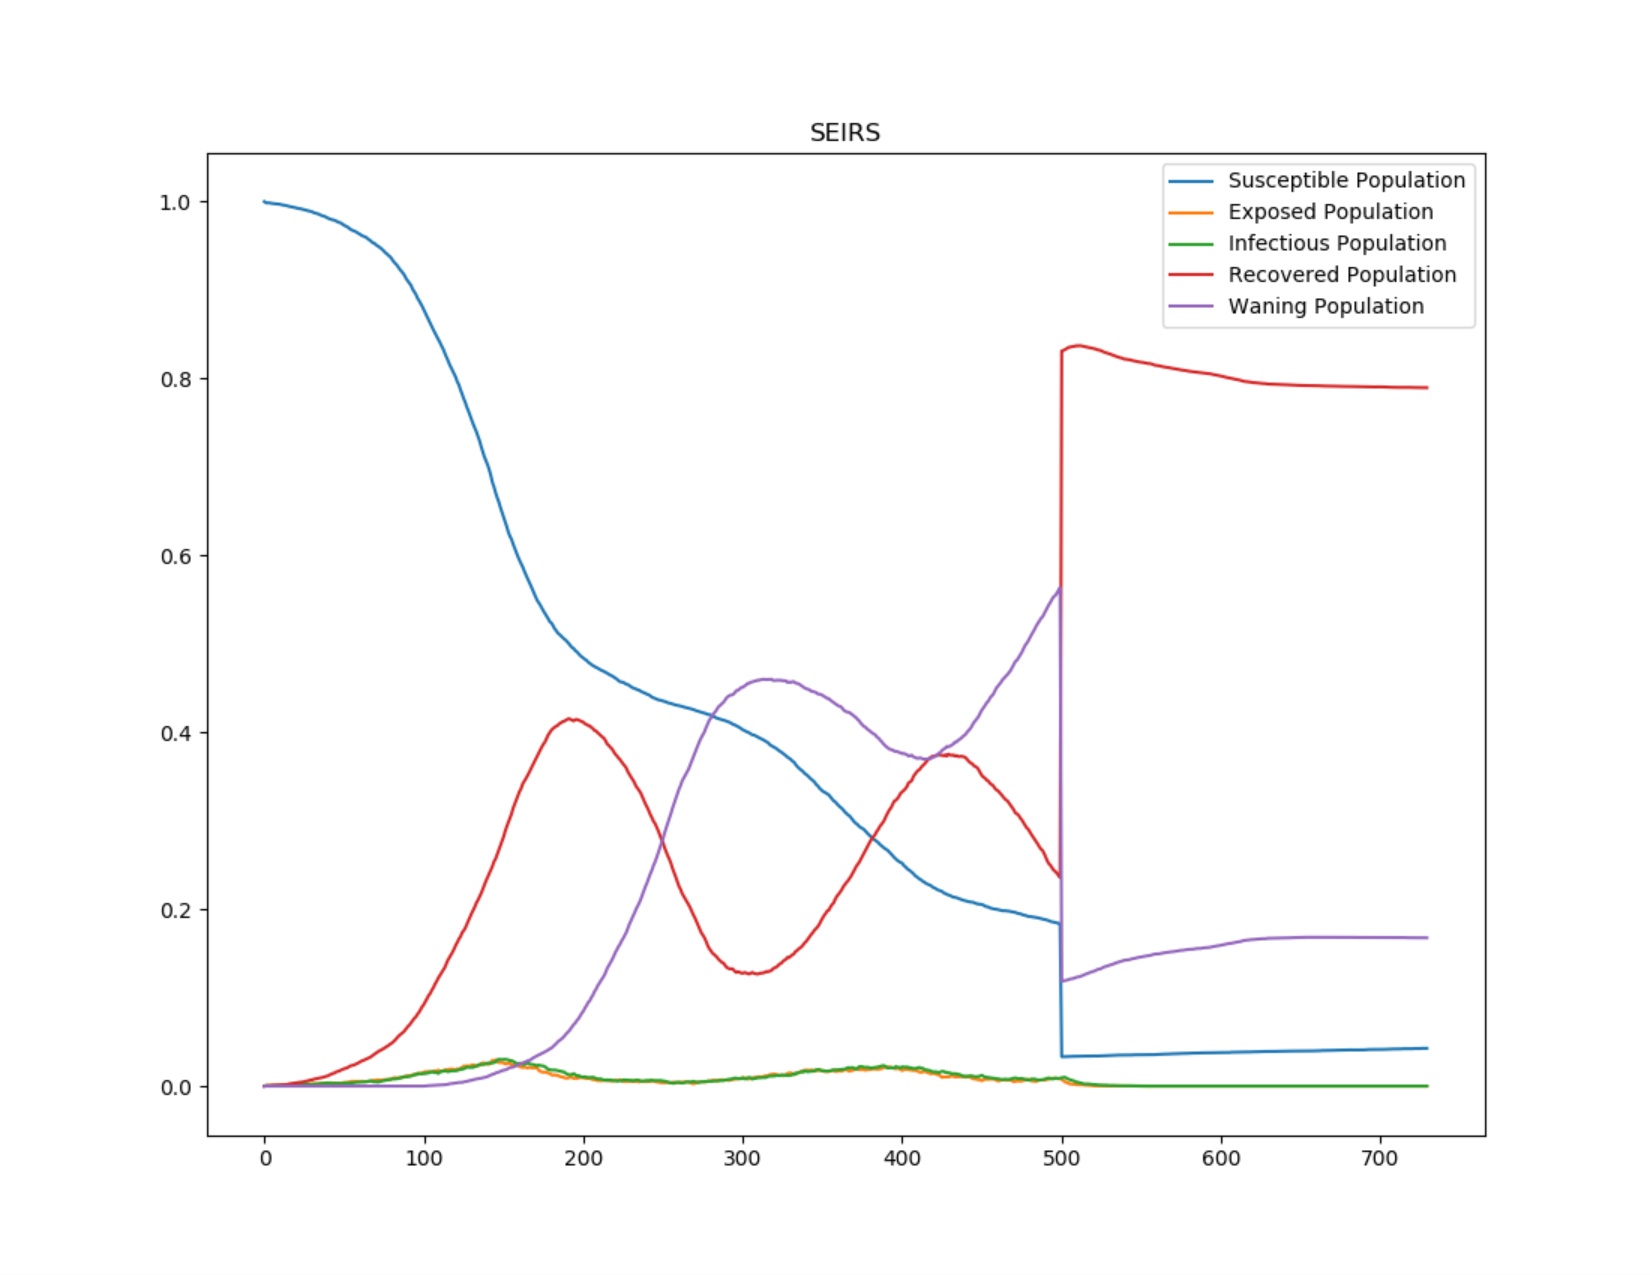
\includegraphics[width=1\textwidth]{SEIRS.png}
\caption{SEIRS}
\end{figure}


\section{Using Package EpiModel}

%from \url{https://timchurches.github.io/blog/posts/2020-03-10-modelling-the-effects-of-public-health-interventions-on-covid-19-transmission-part-1/}

dynamic, continuous-time, compartment models (DCMs), 

stochastic, discrete-time, individual contact models (ICMs)

stochastic, discrete-time, network models



stochastic, discrete-time, individual contact models (ICMs)

\begin{knitrout}
\definecolor{shadecolor}{rgb}{0.969, 0.969, 0.969}\color{fgcolor}\begin{kframe}
\begin{alltt}
\hlstd{control} \hlkwb{<-} \hlkwd{control.icm}\hlstd{(}\hlkwc{type} \hlstd{=} \hlstr{"SIR"}\hlstd{,} \hlkwc{nsteps} \hlstd{=} \hlnum{100}\hlstd{,} \hlkwc{nsims} \hlstd{=} \hlnum{10}\hlstd{)}
\hlstd{init} \hlkwb{<-} \hlkwd{init.icm}\hlstd{(}\hlkwc{s.num} \hlstd{=} \hlnum{997}\hlstd{,} \hlkwc{i.num} \hlstd{=} \hlnum{3}\hlstd{,} \hlkwc{r.num} \hlstd{=} \hlnum{0}\hlstd{)}

\hlstd{param} \hlkwb{<-} \hlkwd{param.icm}\hlstd{(}\hlkwc{inf.prob} \hlstd{=} \hlnum{0.05}\hlstd{,} \hlkwc{act.rate} \hlstd{=} \hlnum{10}\hlstd{,} \hlkwc{rec.rate} \hlstd{=} \hlnum{1}\hlopt{/}\hlnum{20}\hlstd{,}
    \hlkwc{a.rate} \hlstd{= (}\hlnum{10.5}\hlopt{/}\hlnum{365}\hlstd{)}\hlopt{/}\hlnum{1000}\hlstd{,} \hlkwc{ds.rate} \hlstd{= (}\hlnum{7}\hlopt{/}\hlnum{365}\hlstd{)}\hlopt{/}\hlnum{1000}\hlstd{,} \hlkwc{di.rate} \hlstd{= (}\hlnum{14}\hlopt{/}\hlnum{365}\hlstd{)}\hlopt{/}\hlnum{1000}\hlstd{,}
    \hlkwc{dr.rate} \hlstd{= (}\hlnum{7}\hlopt{/}\hlnum{365}\hlstd{)}\hlopt{/}\hlnum{1000}\hlstd{)}
\hlstd{sim} \hlkwb{<-} \hlkwd{icm}\hlstd{(param, init, control)}

\hlstd{sim}
\end{alltt}
\begin{verbatim}
## EpiModel Simulation
## =======================
## Model class: icm
## 
## Simulation Summary
## -----------------------
## Model type: SIR
## No. simulations: 10
## No. time steps: 100
## No. groups: 1
## 
## Model Parameters
## -----------------------
## inf.prob = 0.05
## act.rate = 10
## rec.rate = 0.05
## a.rate = 2.876712e-05
## ds.rate = 1.917808e-05
## di.rate = 3.835616e-05
## dr.rate = 1.917808e-05
## 
## Model Output
## -----------------------
## Variables: s.num i.num num r.num si.flow ir.flow ds.flow 
## di.flow dr.flow a.flow
\end{verbatim}
\end{kframe}
\end{knitrout}


\begin{knitrout}
\definecolor{shadecolor}{rgb}{0.969, 0.969, 0.969}\color{fgcolor}\begin{kframe}
\begin{alltt}
\hlkwd{plot}\hlstd{(sim)}
\end{alltt}
\end{kframe}
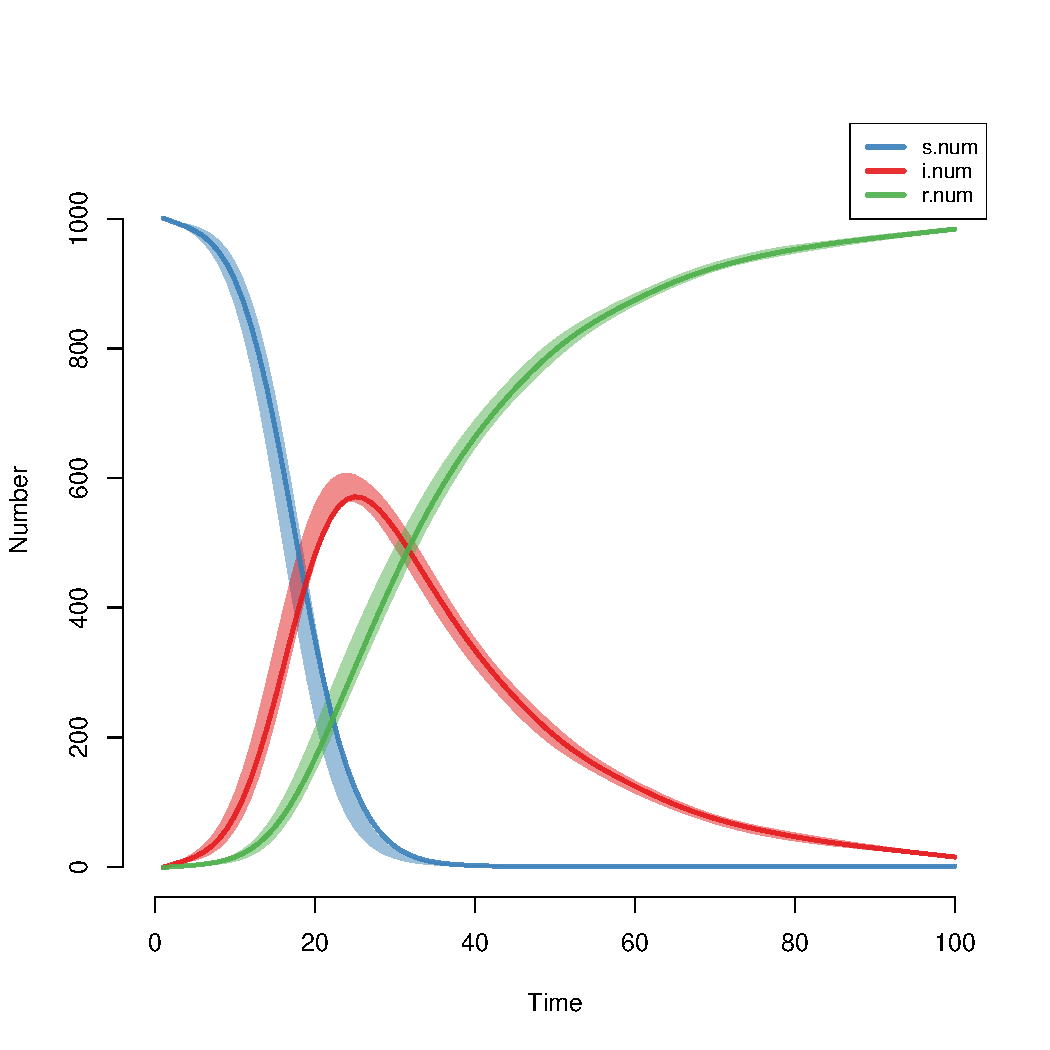
\includegraphics[width=\maxwidth]{figure/unnamed-chunk-12-1} 

\end{knitrout}


\begin{knitrout}
\definecolor{shadecolor}{rgb}{0.969, 0.969, 0.969}\color{fgcolor}\begin{kframe}
\begin{alltt}
\hlkwd{plot}\hlstd{(sim,} \hlkwc{y} \hlstd{=} \hlstr{"si.flow"}\hlstd{,} \hlkwc{mean.col} \hlstd{=} \hlstr{"red"}\hlstd{,} \hlkwc{qnts.col} \hlstd{=} \hlstr{"red"}\hlstd{)}
\end{alltt}
\end{kframe}
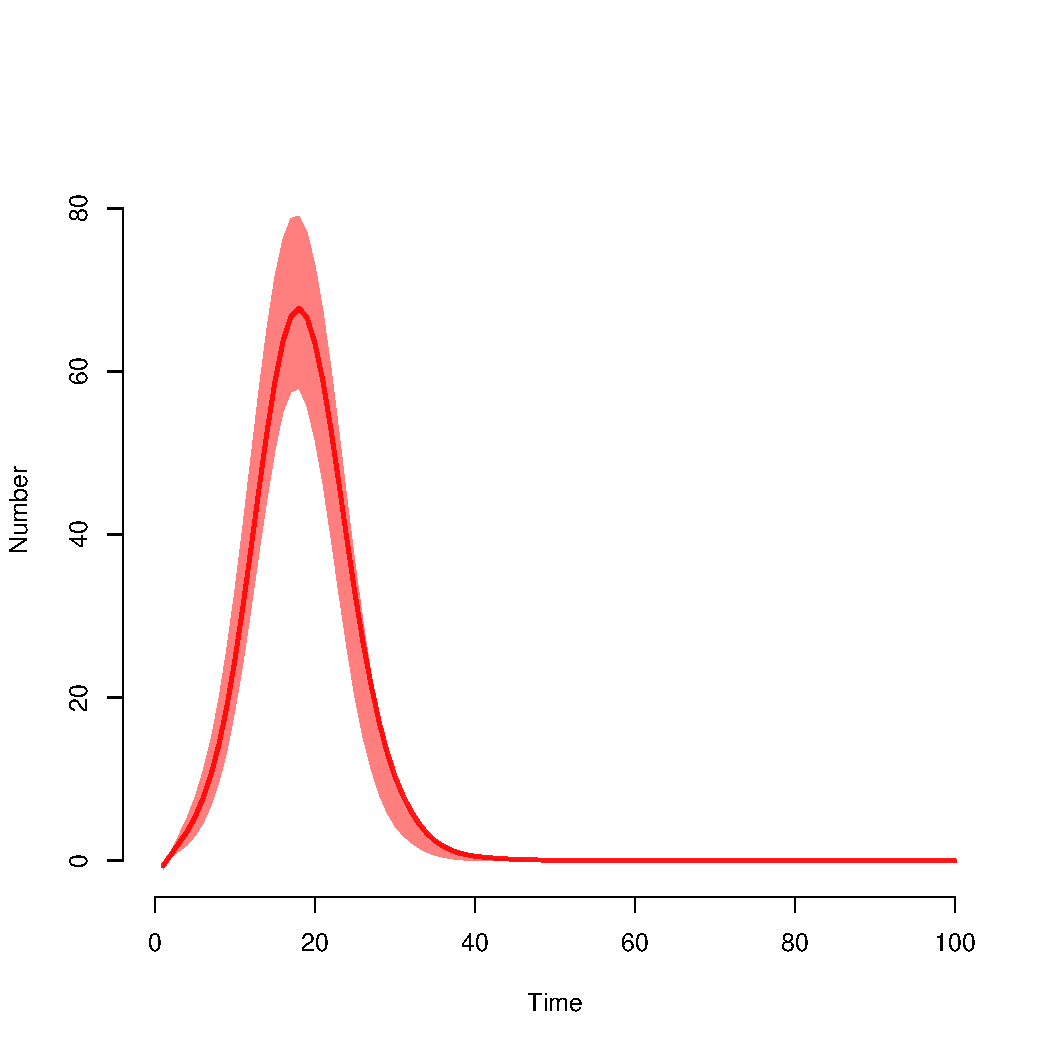
\includegraphics[width=\maxwidth]{figure/unnamed-chunk-13-1} 

\end{knitrout}

\begin{knitrout}
\definecolor{shadecolor}{rgb}{0.969, 0.969, 0.969}\color{fgcolor}\begin{kframe}
\begin{alltt}
\hlstd{run_sir_sim} \hlkwb{<-} \hlkwa{function}\hlstd{(}\hlkwc{inf_prob}\hlstd{,} \hlkwc{act_rate}\hlstd{,} \hlkwc{pop_size} \hlstd{=} \hlnum{1000}\hlstd{,}
    \hlkwc{i_num} \hlstd{=} \hlnum{3}\hlstd{,} \hlkwc{n_steps} \hlstd{=} \hlnum{365}\hlstd{,} \hlkwc{n_sims} \hlstd{=} \hlnum{10}\hlstd{,} \hlkwc{si_mean} \hlstd{=} \hlnum{7.5}\hlstd{,} \hlkwc{si_sd} \hlstd{=} \hlnum{3.4}\hlstd{) \{}

    \hlcom{# set up simulation parameters}
    \hlstd{param} \hlkwb{<-} \hlkwd{param.icm}\hlstd{(}\hlkwc{inf.prob} \hlstd{= inf_prob,} \hlkwc{act.rate} \hlstd{= act_rate,}
        \hlkwc{rec.rate} \hlstd{=} \hlnum{1}\hlopt{/}\hlnum{20}\hlstd{,} \hlkwc{a.rate} \hlstd{= (}\hlnum{10.5}\hlopt{/}\hlnum{365}\hlstd{)}\hlopt{/}\hlnum{1000}\hlstd{,} \hlkwc{ds.rate} \hlstd{= (}\hlnum{7}\hlopt{/}\hlnum{365}\hlstd{)}\hlopt{/}\hlnum{1000}\hlstd{,}
        \hlkwc{di.rate} \hlstd{= (}\hlnum{14}\hlopt{/}\hlnum{365}\hlstd{)}\hlopt{/}\hlnum{1000}\hlstd{,} \hlkwc{dr.rate} \hlstd{= (}\hlnum{7}\hlopt{/}\hlnum{365}\hlstd{)}\hlopt{/}\hlnum{1000}\hlstd{)}
    \hlstd{init} \hlkwb{<-} \hlkwd{init.icm}\hlstd{(}\hlkwc{s.num} \hlstd{= pop_size} \hlopt{-} \hlstd{i_num,} \hlkwc{i.num} \hlstd{= i_num,}
        \hlkwc{r.num} \hlstd{=} \hlnum{0}\hlstd{)}
    \hlstd{control} \hlkwb{<-} \hlkwd{control.icm}\hlstd{(}\hlkwc{type} \hlstd{=} \hlstr{"SIR"}\hlstd{,} \hlkwc{nsteps} \hlstd{= n_steps,} \hlkwc{nsims} \hlstd{= n_sims)}

    \hlcom{# run the simulation}
    \hlstd{sim} \hlkwb{<-} \hlkwd{icm}\hlstd{(param, init, control)}

    \hlcom{# collect the relevant results in a data frame}
    \hlstd{incidence_rates} \hlkwb{<-} \hlkwd{as.data.frame}\hlstd{(sim,} \hlkwc{out} \hlstd{=} \hlstr{"mean"}\hlstd{)} \hlopt \hlkwd{select}\hlstd{(time,}
        \hlstd{si.flow, i.num)} \hlopt \hlkwd{mutate}\hlstd{(}\hlkwc{act_rate} \hlstd{= act_rate,} \hlkwc{inf_prob} \hlstd{= inf_prob,}
        \hlkwc{total_cases} \hlstd{=} \hlkwd{sum}\hlstd{(si.flow),} \hlkwc{max_prev} \hlstd{=} \hlkwd{max}\hlstd{(i.num,} \hlkwc{na.rm} \hlstd{=} \hlnum{TRUE}\hlstd{))}

    \hlcom{# use the data frame of results to create an incidence()}
    \hlcom{# object}
    \hlstd{local_case_dates} \hlkwb{<-} \hlstd{incidence_rates} \hlopt \hlkwd{filter}\hlstd{(time} \hlopt{<=} \hlnum{300}\hlstd{,}
        \hlstd{act.rate} \hlopt{==} \hlstd{act_rate, inf.prob} \hlopt{==} \hlstd{inf_prob)} \hlopt \hlkwd{select}\hlstd{(time,}
        \hlstd{si.flow)} \hlopt \hlkwd{uncount}\hlstd{(si.flow)} \hlopt \hlkwd{pull}\hlstd{(time)}

    \hlkwa{if} \hlstd{(}\hlkwd{length}\hlstd{(local_case_dates)} \hlopt{>} \hlnum{0}\hlstd{) \{}

        \hlstd{local_cases} \hlkwb{<-} \hlstd{local_case_dates} \hlopt \hlkwd{incidence}\hlstd{(.)}

        \hlcom{# find the incidence peak from the incidence object}
        \hlstd{peaky_blinder} \hlkwb{<-} \hlkwd{find_peak}\hlstd{(local_cases)}

        \hlcom{# recreate the incidence object using data only up to the}
        \hlcom{# peak}
        \hlstd{local_growth_phase_case_dates} \hlkwb{<-} \hlstd{incidence_rates} \hlopt
            \hlkwd{filter}\hlstd{(time} \hlopt{<=} \hlstd{peaky_blinder)} \hlopt \hlkwd{select}\hlstd{(time, si.flow)} \hlopt
            \hlkwd{uncount}\hlstd{(si.flow)} \hlopt \hlkwd{pull}\hlstd{(time)}

        \hlstd{local_growth_phase_cases} \hlkwb{<-} \hlstd{local_growth_phase_case_dates} \hlopt
            \hlkwd{incidence}\hlstd{(.,} \hlkwc{last_date} \hlstd{= peaky_blinder)}

        \hlcom{# get a MLE estimate of the basic reproduction number, R0}
        \hlstd{res} \hlkwb{<-} \hlkwd{get_R}\hlstd{(local_growth_phase_cases,} \hlkwc{si_mean} \hlstd{= si_mean,}
            \hlkwc{si_sd} \hlstd{= si_sd)}

        \hlcom{# add that as a column to the data frame of results}
        \hlstd{incidence_rates} \hlkwb{<-} \hlstd{incidence_rates} \hlopt \hlkwd{mutate}\hlstd{(}\hlkwc{mle_R0} \hlstd{= res}\hlopt{$}\hlstd{R_ml)}
    \hlstd{\}} \hlkwa{else} \hlstd{\{}
        \hlcom{# can't calculate R0 so just set to NA}
        \hlstd{incidence_rates} \hlkwb{<-} \hlstd{incidence_rates} \hlopt \hlkwd{mutate}\hlstd{(}\hlkwc{mle_R0} \hlstd{=} \hlnum{NA}\hlstd{)}
    \hlstd{\}}
    \hlcom{# return the data frame (which has just one row)}
    \hlkwd{return}\hlstd{(incidence_rates)}
\hlstd{\}}  \hlcom{# end function definition}
\end{alltt}
\end{kframe}
\end{knitrout}


\begin{knitrout}
\definecolor{shadecolor}{rgb}{0.969, 0.969, 0.969}\color{fgcolor}\begin{kframe}
\begin{alltt}
\hlkwd{library}\hlstd{(earlyR)}
\hlcom{# set up an empty data frame to which to append results from}
\hlcom{# each simulation}
\hlstd{sims_incidence_rates} \hlkwb{<-} \hlkwd{tibble}\hlstd{(}\hlkwc{time} \hlstd{=} \hlkwd{integer}\hlstd{(}\hlnum{0}\hlstd{),} \hlkwc{si.flow} \hlstd{=} \hlkwd{numeric}\hlstd{(}\hlnum{0}\hlstd{),}
    \hlkwc{i.num} \hlstd{=} \hlkwd{numeric}\hlstd{(}\hlnum{0}\hlstd{),} \hlkwc{act_rate} \hlstd{=} \hlkwd{numeric}\hlstd{(}\hlnum{0}\hlstd{),} \hlkwc{inf_prob} \hlstd{=} \hlkwd{numeric}\hlstd{(}\hlnum{0}\hlstd{),}
    \hlkwc{total_cases} \hlstd{=} \hlkwd{numeric}\hlstd{(}\hlnum{0}\hlstd{),} \hlkwc{max_prev} \hlstd{=} \hlkwd{numeric}\hlstd{(}\hlnum{0}\hlstd{),} \hlkwc{mle_R0} \hlstd{=} \hlkwd{numeric}\hlstd{(}\hlnum{0}\hlstd{))}

\hlcom{# the parameters to step through}
\hlstd{act.rates} \hlkwb{<-} \hlkwd{c}\hlstd{(}\hlnum{10}\hlstd{,} \hlnum{5}\hlstd{,} \hlnum{2}\hlstd{)}
\hlstd{inf.probs} \hlkwb{<-} \hlkwd{c}\hlstd{(}\hlnum{0.05}\hlstd{,} \hlnum{0.025}\hlstd{,} \hlnum{0.01}\hlstd{)}

\hlcom{# loop through the parameter space}
\hlkwa{for} \hlstd{(act.rate} \hlkwa{in} \hlstd{act.rates) \{}
    \hlkwa{for} \hlstd{(inf.prob} \hlkwa{in} \hlstd{inf.probs) \{}
        \hlstd{sims_incidence_rates} \hlkwb{<-} \hlstd{sims_incidence_rates} \hlopt \hlkwd{bind_rows}\hlstd{(}\hlkwd{run_sir_sim}\hlstd{(inf.prob,}
            \hlstd{act.rate))}
    \hlstd{\}}
\hlstd{\}}
\end{alltt}
\end{kframe}
\end{knitrout}

\begin{knitrout}
\definecolor{shadecolor}{rgb}{0.969, 0.969, 0.969}\color{fgcolor}\begin{kframe}
\begin{alltt}
\hlcom{# create facet columns as descending ordered factors}
\hlstd{sims_incidence_rates} \hlkwb{<-} \hlstd{sims_incidence_rates} \hlopt \hlkwd{mutate}\hlstd{(}\hlkwc{act_rate_facet_label} \hlstd{=} \hlkwd{paste}\hlstd{(act_rate,}
    \hlstr{"exposures per day"}\hlstd{),} \hlkwc{inf_prob_facet_label} \hlstd{=} \hlkwd{paste}\hlstd{(}\hlstr{"Probability of infection\textbackslash{}nat each exposure:"}\hlstd{,}
    \hlstd{inf_prob))} \hlopt \hlkwd{arrange}\hlstd{(}\hlkwd{desc}\hlstd{(act_rate))} \hlopt \hlkwd{mutate_at}\hlstd{(}\hlkwd{vars}\hlstd{(act_rate_facet_label),}
    \hlkwd{funs}\hlstd{(}\hlkwd{factor}\hlstd{(.,} \hlkwc{levels} \hlstd{=} \hlkwd{unique}\hlstd{(.))))} \hlopt \hlkwd{arrange}\hlstd{(}\hlkwd{desc}\hlstd{(inf_prob))} \hlopt
    \hlkwd{mutate_at}\hlstd{(}\hlkwd{vars}\hlstd{(inf_prob_facet_label),} \hlkwd{funs}\hlstd{(}\hlkwd{factor}\hlstd{(.,} \hlkwc{levels} \hlstd{=} \hlkwd{unique}\hlstd{(.))))} \hlopt
    \hlkwd{arrange}\hlstd{(}\hlkwd{desc}\hlstd{(act_rate),} \hlkwd{desc}\hlstd{(inf_prob), time)}
\end{alltt}


{\ttfamily\noindent\color{warningcolor}{\#\# Warning: funs() is soft deprecated as of dplyr 0.8.0\\\#\# Please use a list of either functions or lambdas: \\\#\# \\\#\#\ \  \# Simple named list: \\\#\#\ \  list(mean = mean, median = median)\\\#\# \\\#\#\ \  \# Auto named with `tibble::lst()`: \\\#\#\ \  tibble::lst(mean, median)\\\#\# \\\#\#\ \  \# Using lambdas\\\#\#\ \  list(\textasciitilde{} mean(., trim = .2), \textasciitilde{} median(., na.rm = TRUE))\\\#\# This warning is displayed once per session.}}\begin{alltt}
\hlcom{# add annotation text for each facet}
\hlstd{sims_incidence_rates_facet_annotations} \hlkwb{<-} \hlstd{sims_incidence_rates} \hlopt
    \hlkwd{mutate}\hlstd{(}\hlkwc{label} \hlstd{=} \hlkwd{paste}\hlstd{(}\hlstr{"R0 ="}\hlstd{,} \hlkwd{format}\hlstd{(mle_R0,} \hlkwc{digits} \hlstd{=} \hlnum{3}\hlstd{),}
        \hlstr{"\textbackslash{}n"}\hlstd{,} \hlkwd{round}\hlstd{(}\hlnum{100} \hlopt{*} \hlstd{total_cases}\hlopt{/}\hlnum{1000}\hlstd{,} \hlkwc{digits} \hlstd{=} \hlnum{0}\hlstd{),} \hlstr{"% of population infected"}\hlstd{))} \hlopt
    \hlkwd{select}\hlstd{(inf_prob_facet_label, act_rate_facet_label, label)} \hlopt
    \hlkwd{distinct}\hlstd{()}

\hlstd{sims_incidence_rates} \hlopt \hlkwd{filter}\hlstd{(time} \hlopt{<=} \hlnum{365}\hlstd{)} \hlopt \hlkwd{ggplot}\hlstd{(}\hlkwd{aes}\hlstd{(}\hlkwc{x} \hlstd{= time,}
    \hlkwc{y} \hlstd{= si.flow))} \hlopt{+} \hlkwd{geom_line}\hlstd{(}\hlkwc{colour} \hlstd{=} \hlstr{"blue"}\hlstd{,} \hlkwc{size} \hlstd{=} \hlnum{1.5}\hlstd{)} \hlopt{+}
    \hlkwd{facet_grid}\hlstd{(inf_prob_facet_label} \hlopt{~} \hlstd{act_rate_facet_label)} \hlopt{+}
    \hlkwd{geom_text}\hlstd{(}\hlkwc{data} \hlstd{= sims_incidence_rates_facet_annotations,}
        \hlkwc{mapping} \hlstd{=} \hlkwd{aes}\hlstd{(}\hlkwc{x} \hlstd{=} \hlnum{50}\hlstd{,} \hlkwc{y} \hlstd{=} \hlnum{0.8} \hlopt{*} \hlkwd{max}\hlstd{(sims_incidence_rates}\hlopt{$}\hlstd{si.flow,}
            \hlkwc{na.rm} \hlstd{=} \hlnum{TRUE}\hlstd{),} \hlkwc{label} \hlstd{= label),} \hlkwc{parse} \hlstd{=} \hlnum{FALSE}\hlstd{,} \hlkwc{hjust} \hlstd{=} \hlnum{0}\hlstd{,}
        \hlkwc{vjust} \hlstd{=} \hlnum{0}\hlstd{,} \hlkwc{size} \hlstd{=} \hlnum{3}\hlstd{)} \hlopt{+} \hlkwd{labs}\hlstd{(}\hlkwc{x} \hlstd{=} \hlstr{"Days since start of epidemic"}\hlstd{,}
    \hlkwc{y} \hlstd{=} \hlstr{"New cases per day"}\hlstd{,} \hlkwc{title} \hlstd{=} \hlstr{"Modelling of new cases of COVID-19 per day: incidence rate"}\hlstd{,}
    \hlkwc{subtitle} \hlstd{=} \hlkwd{paste}\hlstd{(}\hlstr{"with varying levels of social mixing (exposures per day)"}\hlstd{,}
        \hlstr{"and probabilities of infection at each exposure"}\hlstd{))} \hlopt{+}
    \hlkwd{theme}\hlstd{(}\hlkwc{legend.position} \hlstd{=} \hlstr{"top"}\hlstd{,} \hlkwc{strip.text} \hlstd{=} \hlkwd{element_text}\hlstd{(}\hlkwc{size} \hlstd{=} \hlnum{14}\hlstd{))}
\end{alltt}
\end{kframe}
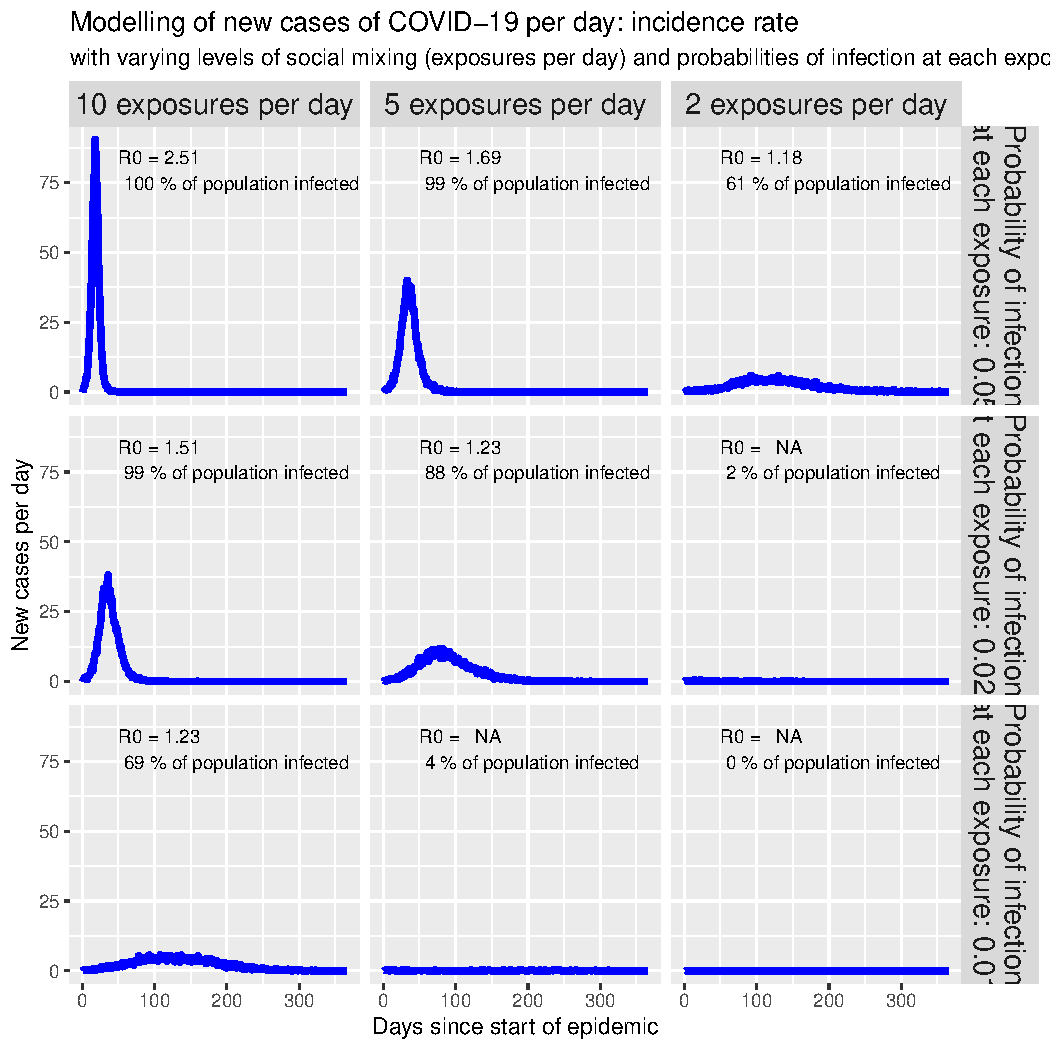
\includegraphics[width=\maxwidth]{figure/unnamed-chunk-16-1} 

\end{knitrout}



\section{SEIQHRF --Wow, now we can model stuff!}

%this is copied from \url{https://timchurches.github.io/blog/posts/2020-03-18-modelling-the-effects-of-public-health-interventions-on-covid-19-transmission-part-2/}

\begin{knitrout}
\definecolor{shadecolor}{rgb}{0.969, 0.969, 0.969}\color{fgcolor}\begin{kframe}
\begin{alltt}
\hlkwd{tic}\hlstd{(}\hlstr{"Time to complete"}\hlstd{)}
\end{alltt}
\end{kframe}
\end{knitrout}

\begin{knitrout}
\definecolor{shadecolor}{rgb}{0.969, 0.969, 0.969}\color{fgcolor}\begin{kframe}
\begin{alltt}
\hlstd{source_files} \hlkwb{<-} \hlkwd{c}\hlstd{(}\hlstr{"_icm.mod.init.seiqhrf.R"}\hlstd{,} \hlstr{"_icm.mod.status.seiqhrf.R"}\hlstd{,}
    \hlstr{"_icm.mod.vital.seiqhrf.R"}\hlstd{,} \hlstr{"_icm.control.seiqhrf.R"}\hlstd{,} \hlstr{"_icm.utils.seiqhrf.R"}\hlstd{,}
    \hlstr{"_icm.saveout.seiqhrf.R"}\hlstd{,} \hlstr{"_icm.icm.seiqhrf.R"}\hlstd{)}

\hlstd{src_path} \hlkwb{<-} \hlkwd{paste0}\hlstd{(}\hlstr{"./_posts/2020-03-18-modelling-the-effects-of-public-health-"}\hlstd{,}
    \hlstr{"interventions-on-covid-19-transmission-part-2/"}\hlstd{)}

\hlstd{gist_url} \hlkwb{<-} \hlstr{"https://gist.github.com/timchurches/92073d0ea75cfbd387f91f7c6e624bd7"}

\hlstd{local_source} \hlkwb{<-} \hlnum{FALSE}

\hlkwa{for} \hlstd{(source_file} \hlkwa{in} \hlstd{source_files) \{}
    \hlkwa{if} \hlstd{(local_source) \{}
        \hlkwd{source}\hlstd{(}\hlkwd{paste}\hlstd{(src_path, source_file,} \hlkwc{sep} \hlstd{=} \hlstr{""}\hlstd{))}
    \hlstd{\}} \hlkwa{else} \hlstd{\{}
        \hlkwd{source_gist}\hlstd{(gist_url,} \hlkwc{filename} \hlstd{= source_file)}
    \hlstd{\}}
\hlstd{\}}
\end{alltt}


{\ttfamily\noindent\itshape\color{messagecolor}{\#\# Sourcing https://gist.githubusercontent.com/timchurches/92073d0ea75cfbd387f91f7c6e624bd7/raw/669fffee6c37fd3345862d56b13b3f30f21e7ea9/\_icm.mod.init.seiqhrf.R}}

{\ttfamily\noindent\itshape\color{messagecolor}{\#\# SHA-1 hash of file is 323250b6e71cd44c3d201fe2b7c85df896a65368}}

{\ttfamily\noindent\itshape\color{messagecolor}{\#\# Sourcing https://gist.githubusercontent.com/timchurches/92073d0ea75cfbd387f91f7c6e624bd7/raw/8b63fae903bf8f83d4a583344c380ed9fac99b81/\_icm.mod.status.seiqhrf.R}}

{\ttfamily\noindent\itshape\color{messagecolor}{\#\# SHA-1 hash of file is 63756c53135ded7eb697831f59aa24b84edda344}}

{\ttfamily\noindent\itshape\color{messagecolor}{\#\# Sourcing https://gist.githubusercontent.com/timchurches/92073d0ea75cfbd387f91f7c6e624bd7/raw/d84384f08c7a7dc4f98c5ba20c84a994d0909501/\_icm.mod.vital.seiqhrf.R}}

{\ttfamily\noindent\itshape\color{messagecolor}{\#\# SHA-1 hash of file is e864b3c4043b8ec22ed65408bfe36d7b75a3afaa}}

{\ttfamily\noindent\itshape\color{messagecolor}{\#\# Sourcing https://gist.githubusercontent.com/timchurches/92073d0ea75cfbd387f91f7c6e624bd7/raw/c3ad4e18811f594f0f373e6d1c45aa3dbbd4cbac/\_icm.control.seiqhrf.R}}

{\ttfamily\noindent\itshape\color{messagecolor}{\#\# SHA-1 hash of file is 8514ecf3080ca0b96d53d3d81e0019af4cdd1c07}}

{\ttfamily\noindent\itshape\color{messagecolor}{\#\# Sourcing https://gist.githubusercontent.com/timchurches/92073d0ea75cfbd387f91f7c6e624bd7/raw/f87f429340386f92246340aeffa669997b9ac3a1/\_icm.utils.seiqhrf.R}}

{\ttfamily\noindent\itshape\color{messagecolor}{\#\# SHA-1 hash of file is cfd032f1285332f8c4d2cc1a13c8c92920ae9370}}

{\ttfamily\noindent\itshape\color{messagecolor}{\#\# Sourcing https://gist.githubusercontent.com/timchurches/92073d0ea75cfbd387f91f7c6e624bd7/raw/de23f19a93f82585bceecd31a47b4be9dec802e8/\_icm.saveout.seiqhrf.R}}

{\ttfamily\noindent\itshape\color{messagecolor}{\#\# SHA-1 hash of file is 14b18703fc9e46d31e279a364df4e89369ddae98}}

{\ttfamily\noindent\itshape\color{messagecolor}{\#\# Sourcing https://gist.githubusercontent.com/timchurches/92073d0ea75cfbd387f91f7c6e624bd7/raw/824302a1c10a353e1dce47e6f53d3a73ebac9849/\_icm.icm.seiqhrf.R}}

{\ttfamily\noindent\itshape\color{messagecolor}{\#\# SHA-1 hash of file is 182364e711588462e32ff3254947027f78c920ed}}\end{kframe}
\end{knitrout}


\begin{knitrout}
\definecolor{shadecolor}{rgb}{0.969, 0.969, 0.969}\color{fgcolor}\begin{kframe}
\begin{alltt}
\hlcom{# function to set-up and run the baseline simulations}
\hlstd{simulate} \hlkwb{<-} \hlkwa{function}\hlstd{(}\hlcom{# control.icm params}
                     \hlkwc{type} \hlstd{=} \hlstr{"SEIQHRF"}\hlstd{,}
                     \hlkwc{nsteps} \hlstd{=} \hlnum{366}\hlstd{,}
                     \hlkwc{nsims} \hlstd{=} \hlnum{8}\hlstd{,}
                     \hlkwc{ncores} \hlstd{=} \hlnum{4}\hlstd{,}
                     \hlkwc{prog.rand} \hlstd{=} \hlnum{FALSE}\hlstd{,}
                     \hlkwc{rec.rand} \hlstd{=} \hlnum{FALSE}\hlstd{,}
                     \hlkwc{fat.rand} \hlstd{=} \hlnum{TRUE}\hlstd{,}
                     \hlkwc{quar.rand} \hlstd{=} \hlnum{FALSE}\hlstd{,}
                     \hlkwc{hosp.rand} \hlstd{=} \hlnum{FALSE}\hlstd{,}
                     \hlkwc{disch.rand} \hlstd{=} \hlnum{TRUE}\hlstd{,}
                     \hlkwc{infection.FUN} \hlstd{= infection.seiqhrf.icm,}
                     \hlkwc{recovery.FUN} \hlstd{= progress.seiqhrf.icm,}
                     \hlkwc{departures.FUN} \hlstd{= departures.seiqhrf.icm,}
                     \hlkwc{arrivals.FUN} \hlstd{= arrivals.icm,}
                     \hlkwc{get_prev.FUN} \hlstd{= get_prev.seiqhrf.icm,}
                     \hlcom{# init.icm params}
                     \hlkwc{s.num} \hlstd{=} \hlnum{9997}\hlstd{,}
                     \hlkwc{e.num}\hlstd{=}\hlnum{0}\hlstd{,}
                     \hlkwc{i.num} \hlstd{=} \hlnum{3}\hlstd{,}
                     \hlkwc{q.num}\hlstd{=}\hlnum{0}\hlstd{,}
                     \hlkwc{h.num}\hlstd{=}\hlnum{0}\hlstd{,}
                     \hlkwc{r.num} \hlstd{=} \hlnum{0}\hlstd{,}
                     \hlkwc{f.num} \hlstd{=} \hlnum{0}\hlstd{,}
                     \hlcom{# param.icm params}
                     \hlkwc{inf.prob.e} \hlstd{=} \hlnum{0.02}\hlstd{,}
                     \hlkwc{act.rate.e} \hlstd{=} \hlnum{10}\hlstd{,}
                     \hlkwc{inf.prob.i} \hlstd{=} \hlnum{0.05}\hlstd{,}
                     \hlkwc{act.rate.i} \hlstd{=} \hlnum{10}\hlstd{,}
                     \hlkwc{inf.prob.q} \hlstd{=} \hlnum{0.02}\hlstd{,}
                     \hlkwc{act.rate.q} \hlstd{=} \hlnum{2.5}\hlstd{,}
                     \hlkwc{quar.rate} \hlstd{=} \hlnum{1}\hlopt{/}\hlnum{30}\hlstd{,}
                     \hlkwc{hosp.rate} \hlstd{=} \hlnum{1}\hlopt{/}\hlnum{100}\hlstd{,}
                     \hlkwc{disch.rate} \hlstd{=} \hlnum{1}\hlopt{/}\hlnum{15}\hlstd{,}
                     \hlkwc{prog.rate} \hlstd{=} \hlnum{1}\hlopt{/}\hlnum{10}\hlstd{,}
                     \hlkwc{prog.dist.scale} \hlstd{=} \hlnum{5}\hlstd{,}
                     \hlkwc{prog.dist.shape} \hlstd{=} \hlnum{1.5}\hlstd{,}
                     \hlkwc{rec.rate} \hlstd{=} \hlnum{1}\hlopt{/}\hlnum{20}\hlstd{,}
                     \hlkwc{rec.dist.scale} \hlstd{=} \hlnum{35}\hlstd{,}
                     \hlkwc{rec.dist.shape} \hlstd{=} \hlnum{1.5}\hlstd{,}
                     \hlkwc{fat.rate.base} \hlstd{=} \hlnum{1}\hlopt{/}\hlnum{50}\hlstd{,}
                     \hlkwc{hosp.cap} \hlstd{=} \hlnum{40}\hlstd{,}
                     \hlkwc{fat.rate.overcap} \hlstd{=} \hlnum{1}\hlopt{/}\hlnum{25}\hlstd{,}
                     \hlkwc{fat.tcoeff} \hlstd{=} \hlnum{0.5}\hlstd{,}
                     \hlkwc{vital} \hlstd{=} \hlnum{TRUE}\hlstd{,}
                     \hlkwc{a.rate} \hlstd{= (}\hlnum{10.5}\hlopt{/}\hlnum{365}\hlstd{)}\hlopt{/}\hlnum{1000}\hlstd{,}
                     \hlkwc{a.prop.e} \hlstd{=} \hlnum{0.01}\hlstd{,}
                     \hlkwc{a.prop.i} \hlstd{=} \hlnum{0.001}\hlstd{,}
                     \hlkwc{a.prop.q} \hlstd{=} \hlnum{0.01}\hlstd{,}
                     \hlkwc{ds.rate} \hlstd{= (}\hlnum{7}\hlopt{/}\hlnum{365}\hlstd{)}\hlopt{/}\hlnum{1000}\hlstd{,}
                     \hlkwc{de.rate} \hlstd{= (}\hlnum{7}\hlopt{/}\hlnum{365}\hlstd{)}\hlopt{/}\hlnum{1000}\hlstd{,}
                     \hlkwc{di.rate} \hlstd{= (}\hlnum{7}\hlopt{/}\hlnum{365}\hlstd{)}\hlopt{/}\hlnum{1000}\hlstd{,}
                     \hlkwc{dq.rate} \hlstd{= (}\hlnum{7}\hlopt{/}\hlnum{365}\hlstd{)}\hlopt{/}\hlnum{1000}\hlstd{,}
                     \hlkwc{dh.rate} \hlstd{= (}\hlnum{20}\hlopt{/}\hlnum{365}\hlstd{)}\hlopt{/}\hlnum{1000}\hlstd{,}
                     \hlkwc{dr.rate} \hlstd{= (}\hlnum{7}\hlopt{/}\hlnum{365}\hlstd{)}\hlopt{/}\hlnum{1000}\hlstd{,}
                     \hlkwc{out}\hlstd{=}\hlstr{"mean"}
                    \hlstd{) \{}

  \hlstd{control} \hlkwb{<-} \hlkwd{control.icm}\hlstd{(}\hlkwc{type} \hlstd{= type,}
                         \hlkwc{nsteps} \hlstd{= nsteps,}
                         \hlkwc{nsims} \hlstd{= nsims,}
                         \hlkwc{ncores} \hlstd{= ncores,}
                         \hlkwc{prog.rand} \hlstd{= prog.rand,}
                         \hlkwc{rec.rand} \hlstd{= rec.rand,}
                         \hlkwc{infection.FUN} \hlstd{= infection.FUN,}
                         \hlkwc{recovery.FUN} \hlstd{= recovery.FUN,}
                         \hlkwc{arrivals.FUN} \hlstd{= arrivals.FUN,}
                         \hlkwc{departures.FUN} \hlstd{= departures.FUN,}
                         \hlkwc{get_prev.FUN} \hlstd{= get_prev.FUN)}

  \hlstd{init} \hlkwb{<-} \hlkwd{init.icm}\hlstd{(}\hlkwc{s.num} \hlstd{= s.num,}
                   \hlkwc{e.num} \hlstd{= e.num,}
                   \hlkwc{i.num} \hlstd{= i.num,}
                   \hlkwc{q.num} \hlstd{= q.num,}
                   \hlkwc{h.num} \hlstd{= h.num,}
                   \hlkwc{r.num} \hlstd{= r.num,}
                   \hlkwc{f.num} \hlstd{= f.num)}

  \hlstd{param} \hlkwb{<-}  \hlkwd{param.icm}\hlstd{(}\hlkwc{inf.prob.e} \hlstd{= inf.prob.e,}
                      \hlkwc{act.rate.e} \hlstd{= act.rate.e,}
                      \hlkwc{inf.prob.i} \hlstd{= inf.prob.i,}
                      \hlkwc{act.rate.i} \hlstd{= act.rate.i,}
                      \hlkwc{inf.prob.q} \hlstd{= inf.prob.q,}
                      \hlkwc{act.rate.q} \hlstd{= act.rate.q,}
                      \hlkwc{quar.rate} \hlstd{= quar.rate,}
                      \hlkwc{hosp.rate} \hlstd{= hosp.rate,}
                      \hlkwc{disch.rate} \hlstd{= disch.rate,}
                      \hlkwc{prog.rate} \hlstd{= prog.rate,}
                      \hlkwc{prog.dist.scale} \hlstd{= prog.dist.scale,}
                      \hlkwc{prog.dist.shape} \hlstd{= prog.dist.shape,}
                      \hlkwc{rec.rate} \hlstd{= rec.rate,}
                      \hlkwc{rec.dist.scale} \hlstd{= rec.dist.scale,}
                      \hlkwc{rec.dist.shape} \hlstd{= rec.dist.shape,}
                      \hlkwc{fat.rate.base} \hlstd{= fat.rate.base,}
                      \hlkwc{hosp.cap} \hlstd{= hosp.cap,}
                      \hlkwc{fat.rate.overcap} \hlstd{= fat.rate.overcap,}
                      \hlkwc{fat.tcoeff} \hlstd{= fat.tcoeff,}
                      \hlkwc{vital} \hlstd{= vital,}
                      \hlkwc{a.rate} \hlstd{= a.rate,}
                      \hlkwc{a.prop.e} \hlstd{= a.prop.e,}
                      \hlkwc{a.prop.i} \hlstd{= a.prop.i,}
                      \hlkwc{a.prop.q} \hlstd{= a.prop.q,}
                      \hlkwc{ds.rate} \hlstd{= ds.rate,}
                      \hlkwc{de.rate} \hlstd{= de.rate,}
                      \hlkwc{di.rate} \hlstd{= di.rate,}
                      \hlkwc{dq.rate} \hlstd{= dq.rate,}
                      \hlkwc{dh.rate} \hlstd{= dh.rate,}
                      \hlkwc{dr.rate} \hlstd{= dr.rate)}

  \hlstd{sim} \hlkwb{<-} \hlkwd{icm.seiqhrf}\hlstd{(param, init, control)}
  \hlstd{sim_df} \hlkwb{<-} \hlkwd{as.data.frame}\hlstd{(sim,} \hlkwc{out}\hlstd{=out)}

  \hlkwd{return}\hlstd{(}\hlkwd{list}\hlstd{(}\hlkwc{sim}\hlstd{=sim,} \hlkwc{df}\hlstd{=sim_df))}
\hlstd{\}}
\end{alltt}
\end{kframe}
\end{knitrout}


\begin{knitrout}
\definecolor{shadecolor}{rgb}{0.969, 0.969, 0.969}\color{fgcolor}\begin{kframe}
\begin{alltt}
\hlcom{# define a function to extract timings and assemble a data}
\hlcom{# frame}
\hlstd{get_times} \hlkwb{<-} \hlkwa{function}\hlstd{(}\hlkwc{simulate_results}\hlstd{) \{}

    \hlstd{sim} \hlkwb{<-} \hlstd{simulate_results}\hlopt{$}\hlstd{sim}

    \hlkwa{for} \hlstd{(s} \hlkwa{in} \hlnum{1}\hlopt{:}\hlstd{sim}\hlopt{$}\hlstd{control}\hlopt{$}\hlstd{nsims) \{}
        \hlkwa{if} \hlstd{(s} \hlopt{==} \hlnum{1}\hlstd{) \{}
            \hlstd{times} \hlkwb{<-} \hlstd{sim}\hlopt{$}\hlstd{times[[}\hlkwd{paste}\hlstd{(}\hlstr{"sim"}\hlstd{, s,} \hlkwc{sep} \hlstd{=} \hlstr{""}\hlstd{)]]}
            \hlstd{times} \hlkwb{<-} \hlstd{times} \hlopt \hlkwd{mutate}\hlstd{(}\hlkwc{s} \hlstd{= s)}
        \hlstd{\}} \hlkwa{else} \hlstd{\{}
            \hlstd{times} \hlkwb{<-} \hlstd{times} \hlopt \hlkwd{bind_rows}\hlstd{(sim}\hlopt{$}\hlstd{times[[}\hlkwd{paste}\hlstd{(}\hlstr{"sim"}\hlstd{,}
                \hlstd{s,} \hlkwc{sep} \hlstd{=} \hlstr{""}\hlstd{)]]} \hlopt \hlkwd{mutate}\hlstd{(}\hlkwc{s} \hlstd{= s))}
        \hlstd{\}}
    \hlstd{\}}

    \hlstd{times} \hlkwb{<-} \hlstd{times} \hlopt \hlkwd{mutate}\hlstd{(}\hlkwc{infTime} \hlstd{=} \hlkwd{ifelse}\hlstd{(infTime} \hlopt{<} \hlnum{0}\hlstd{,} \hlopt{-}\hlnum{5}\hlstd{,}
        \hlstd{infTime),} \hlkwc{expTime} \hlstd{=} \hlkwd{ifelse}\hlstd{(expTime} \hlopt{<} \hlnum{0}\hlstd{,} \hlopt{-}\hlnum{5}\hlstd{, expTime))} \hlopt
        \hlkwd{mutate}\hlstd{(}\hlkwc{incubation_period} \hlstd{= infTime} \hlopt{-} \hlstd{expTime,} \hlkwc{illness_duration} \hlstd{= recovTime} \hlopt{-}
            \hlstd{expTime,} \hlkwc{illness_duration_hosp} \hlstd{= dischTime} \hlopt{-} \hlstd{expTime,}
            \hlkwc{hosp_los} \hlstd{= dischTime} \hlopt{-} \hlstd{hospTime,} \hlkwc{quarantine_delay} \hlstd{= quarTime} \hlopt{-}
                \hlstd{infTime,} \hlkwc{survival_time} \hlstd{= fatTime} \hlopt{-} \hlstd{infTime)} \hlopt
        \hlkwd{select}\hlstd{(s, incubation_period, quarantine_delay, illness_duration,}
            \hlstd{illness_duration_hosp, hosp_los, survival_time)} \hlopt
        \hlkwd{pivot_longer}\hlstd{(}\hlopt{-}\hlstd{s,} \hlkwc{names_to} \hlstd{=} \hlstr{"period_type"}\hlstd{,} \hlkwc{values_to} \hlstd{=} \hlstr{"duration"}\hlstd{)} \hlopt
        \hlkwd{mutate}\hlstd{(}\hlkwc{period_type} \hlstd{=} \hlkwd{factor}\hlstd{(period_type,} \hlkwc{levels} \hlstd{=} \hlkwd{c}\hlstd{(}\hlstr{"incubation_period"}\hlstd{,}
            \hlstr{"quarantine_delay"}\hlstd{,} \hlstr{"illness_duration"}\hlstd{,} \hlstr{"illness_duration_hosp"}\hlstd{,}
            \hlstr{"hosp_los"}\hlstd{,} \hlstr{"survival_time"}\hlstd{),} \hlkwc{labels} \hlstd{=} \hlkwd{c}\hlstd{(}\hlstr{"Incubation period"}\hlstd{,}
            \hlstr{"Delay entering isolation"}\hlstd{,} \hlstr{"Illness duration"}\hlstd{,} \hlstr{"Illness duration (hosp)"}\hlstd{,}
            \hlstr{"Hospital care required duration"}\hlstd{,} \hlstr{"Survival time of case fatalities"}\hlstd{),}
            \hlkwc{ordered} \hlstd{=} \hlnum{TRUE}\hlstd{))}
    \hlkwd{return}\hlstd{(times)}
\hlstd{\}}
\end{alltt}
\end{kframe}
\end{knitrout}

\begin{knitrout}
\definecolor{shadecolor}{rgb}{0.969, 0.969, 0.969}\color{fgcolor}\begin{kframe}
\begin{alltt}
\hlstd{times} \hlkwb{<-} \hlkwd{get_times}\hlstd{(baseline_sim)}
\end{alltt}


{\ttfamily\noindent\bfseries\color{errorcolor}{\#\# Error in get\_times(baseline\_sim): object 'baseline\_sim' not found}}\end{kframe}
\end{knitrout}

\begin{knitrout}
\definecolor{shadecolor}{rgb}{0.969, 0.969, 0.969}\color{fgcolor}\begin{kframe}
\begin{alltt}
\hlstd{times} \hlopt \hlkwd{filter}\hlstd{(duration} \hlopt{<=} \hlnum{30}\hlstd{)} \hlopt \hlkwd{ggplot}\hlstd{(}\hlkwd{aes}\hlstd{(}\hlkwc{x} \hlstd{= duration))} \hlopt{+}
    \hlkwd{geom_bar}\hlstd{()} \hlopt{+} \hlkwd{facet_grid}\hlstd{(period_type} \hlopt{~} \hlstd{.,} \hlkwc{scales} \hlstd{=} \hlstr{"free_y"}\hlstd{)} \hlopt{+}
    \hlkwd{labs}\hlstd{(}\hlkwc{title} \hlstd{=} \hlstr{"Duration frequency distributions"}\hlstd{,} \hlkwc{subtitle} \hlstd{=} \hlstr{"Baseline simulation"}\hlstd{)}
\end{alltt}


{\ttfamily\noindent\bfseries\color{errorcolor}{\#\# Error in UseMethod("{}filter\_"{}): no applicable method for 'filter\_' applied to an object of class "{}c('double', 'numeric')"{}}}\end{kframe}
\end{knitrout}

\begin{knitrout}
\definecolor{shadecolor}{rgb}{0.969, 0.969, 0.969}\color{fgcolor}\begin{kframe}
\begin{alltt}
\hlstd{baseline_sim} \hlkwb{<-} \hlkwd{simulate}\hlstd{(}\hlkwc{ncores} \hlstd{=} \hlnum{4}\hlstd{)}
\end{alltt}
\end{kframe}
\end{knitrout}

\begin{knitrout}
\definecolor{shadecolor}{rgb}{0.969, 0.969, 0.969}\color{fgcolor}\begin{kframe}
\begin{alltt}
\hlstd{baseline_plot_df} \hlkwb{<-} \hlstd{baseline_sim}\hlopt{$}\hlstd{df} \hlopt \hlcom{# use only the prevalence columns}
\hlkwd{select}\hlstd{(time, s.num, e.num, i.num, q.num, h.num, r.num, f.num)} \hlopt
    \hlcom{# examine only the first 100 days since it is all over by}
\hlcom{# then using the default parameters}
\hlkwd{filter}\hlstd{(time} \hlopt{<=} \hlnum{100}\hlstd{)} \hlopt \hlkwd{pivot_longer}\hlstd{(}\hlopt{-}\hlkwd{c}\hlstd{(time),} \hlkwc{names_to} \hlstd{=} \hlstr{"compartment"}\hlstd{,}
    \hlkwc{values_to} \hlstd{=} \hlstr{"count"}\hlstd{)}

\hlcom{# define a standard set of colours to represent compartments}
\hlstd{compcols} \hlkwb{<-} \hlkwd{c}\hlstd{(}\hlkwc{s.num} \hlstd{=} \hlstr{"yellow"}\hlstd{,} \hlkwc{e.num} \hlstd{=} \hlstr{"orange"}\hlstd{,} \hlkwc{i.num} \hlstd{=} \hlstr{"red"}\hlstd{,}
    \hlkwc{q.num} \hlstd{=} \hlstr{"cyan"}\hlstd{,} \hlkwc{h.num} \hlstd{=} \hlstr{"magenta"}\hlstd{,} \hlkwc{r.num} \hlstd{=} \hlstr{"lightgreen"}\hlstd{,}
    \hlkwc{f.num} \hlstd{=} \hlstr{"black"}\hlstd{)}
\hlstd{complabels} \hlkwb{<-} \hlkwd{c}\hlstd{(}\hlkwc{s.num} \hlstd{=} \hlstr{"Susceptible"}\hlstd{,} \hlkwc{e.num} \hlstd{=} \hlstr{"Infected/asymptomatic"}\hlstd{,}
    \hlkwc{i.num} \hlstd{=} \hlstr{"Infected/infectious"}\hlstd{,} \hlkwc{q.num} \hlstd{=} \hlstr{"Self-isolated"}\hlstd{,} \hlkwc{h.num} \hlstd{=} \hlstr{"Requires hospitalisation"}\hlstd{,}
    \hlkwc{r.num} \hlstd{=} \hlstr{"Recovered"}\hlstd{,} \hlkwc{f.num} \hlstd{=} \hlstr{"Case fatality"}\hlstd{)}

\hlstd{baseline_plot_df} \hlopt \hlkwd{ggplot}\hlstd{(}\hlkwd{aes}\hlstd{(}\hlkwc{x} \hlstd{= time,} \hlkwc{y} \hlstd{= count,} \hlkwc{colour} \hlstd{= compartment))} \hlopt{+}
    \hlkwd{geom_line}\hlstd{(}\hlkwc{size} \hlstd{=} \hlnum{2}\hlstd{,} \hlkwc{alpha} \hlstd{=} \hlnum{0.7}\hlstd{)} \hlopt{+} \hlkwd{scale_colour_manual}\hlstd{(}\hlkwc{values} \hlstd{= compcols,}
    \hlkwc{labels} \hlstd{= complabels)} \hlopt{+} \hlkwd{theme_dark}\hlstd{()} \hlopt{+} \hlkwd{labs}\hlstd{(}\hlkwc{title} \hlstd{=} \hlstr{"Baseline simulation"}\hlstd{,}
    \hlkwc{x} \hlstd{=} \hlstr{"Days since beginning of epidemic"}\hlstd{,} \hlkwc{y} \hlstd{=} \hlstr{"Prevalence (persons)"}\hlstd{)}
\end{alltt}


{\ttfamily\noindent\color{warningcolor}{\#\# Warning: Removed 5 row(s) containing missing values (geom\_path).}}\end{kframe}
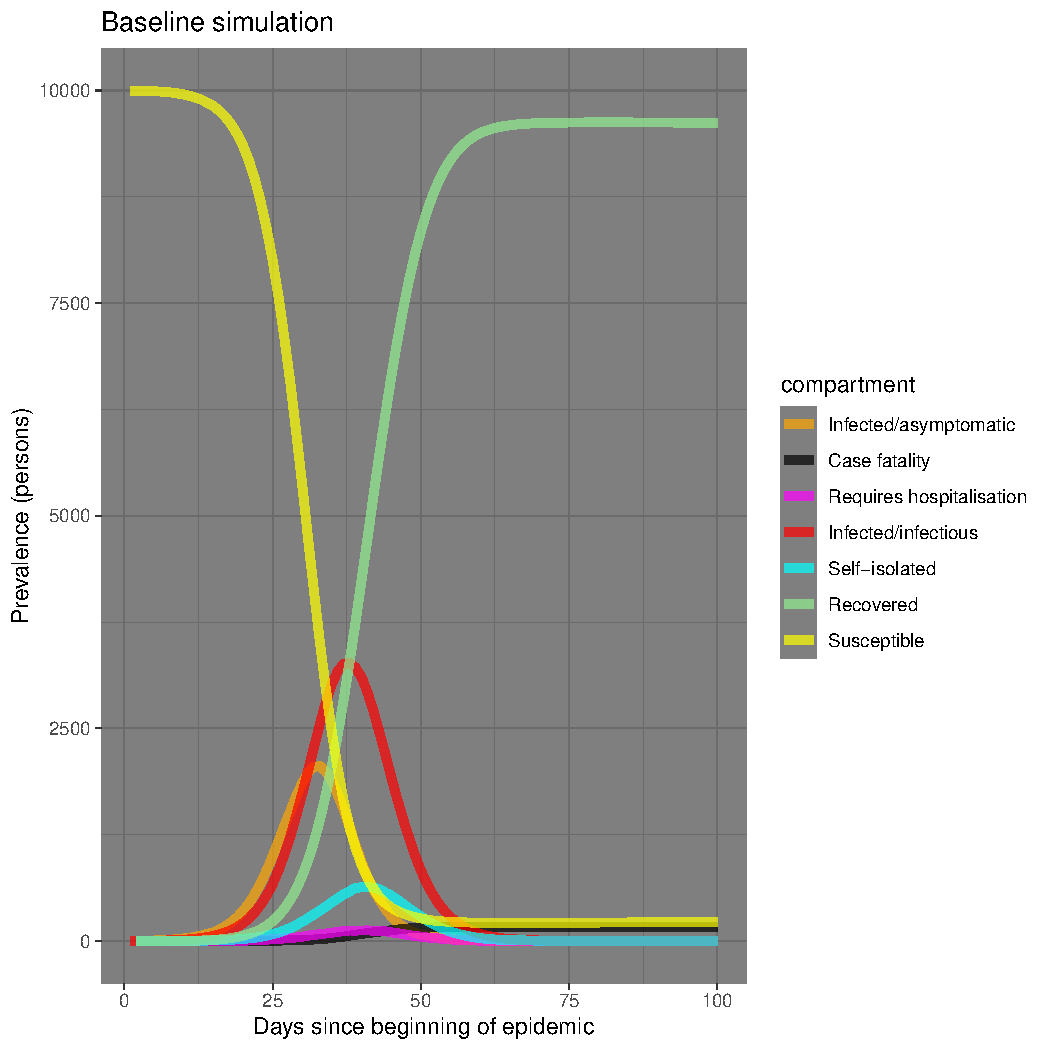
\includegraphics[width=\maxwidth]{figure/unnamed-chunk-24-1} 

\end{knitrout}

\begin{knitrout}
\definecolor{shadecolor}{rgb}{0.969, 0.969, 0.969}\color{fgcolor}\begin{kframe}
\begin{alltt}
\hlstd{baseline_plot_df} \hlopt \hlkwd{filter}\hlstd{(compartment} \hlopt \hlkwd{c}\hlstd{(}\hlstr{"e.num"}\hlstd{,} \hlstr{"i.num"}\hlstd{,}
    \hlstr{"q.num"}\hlstd{,} \hlstr{"h.num"}\hlstd{,} \hlstr{"f.num"}\hlstd{))} \hlopt \hlkwd{ggplot}\hlstd{(}\hlkwd{aes}\hlstd{(}\hlkwc{x} \hlstd{= time,} \hlkwc{y} \hlstd{= count,}
    \hlkwc{colour} \hlstd{= compartment))} \hlopt{+} \hlkwd{geom_line}\hlstd{(}\hlkwc{size} \hlstd{=} \hlnum{2}\hlstd{,} \hlkwc{alpha} \hlstd{=} \hlnum{0.7}\hlstd{)} \hlopt{+}
    \hlkwd{scale_colour_manual}\hlstd{(}\hlkwc{values} \hlstd{= compcols,} \hlkwc{labels} \hlstd{= complabels)} \hlopt{+}
    \hlkwd{theme_dark}\hlstd{()} \hlopt{+} \hlkwd{labs}\hlstd{(}\hlkwc{title} \hlstd{=} \hlstr{"Baseline simulation"}\hlstd{,} \hlkwc{x} \hlstd{=} \hlstr{"Days since beginning of epidemic"}\hlstd{,}
    \hlkwc{y} \hlstd{=} \hlstr{"Prevalence (persons)"}\hlstd{)}
\end{alltt}


{\ttfamily\noindent\color{warningcolor}{\#\# Warning: Removed 4 row(s) containing missing values (geom\_path).}}\end{kframe}
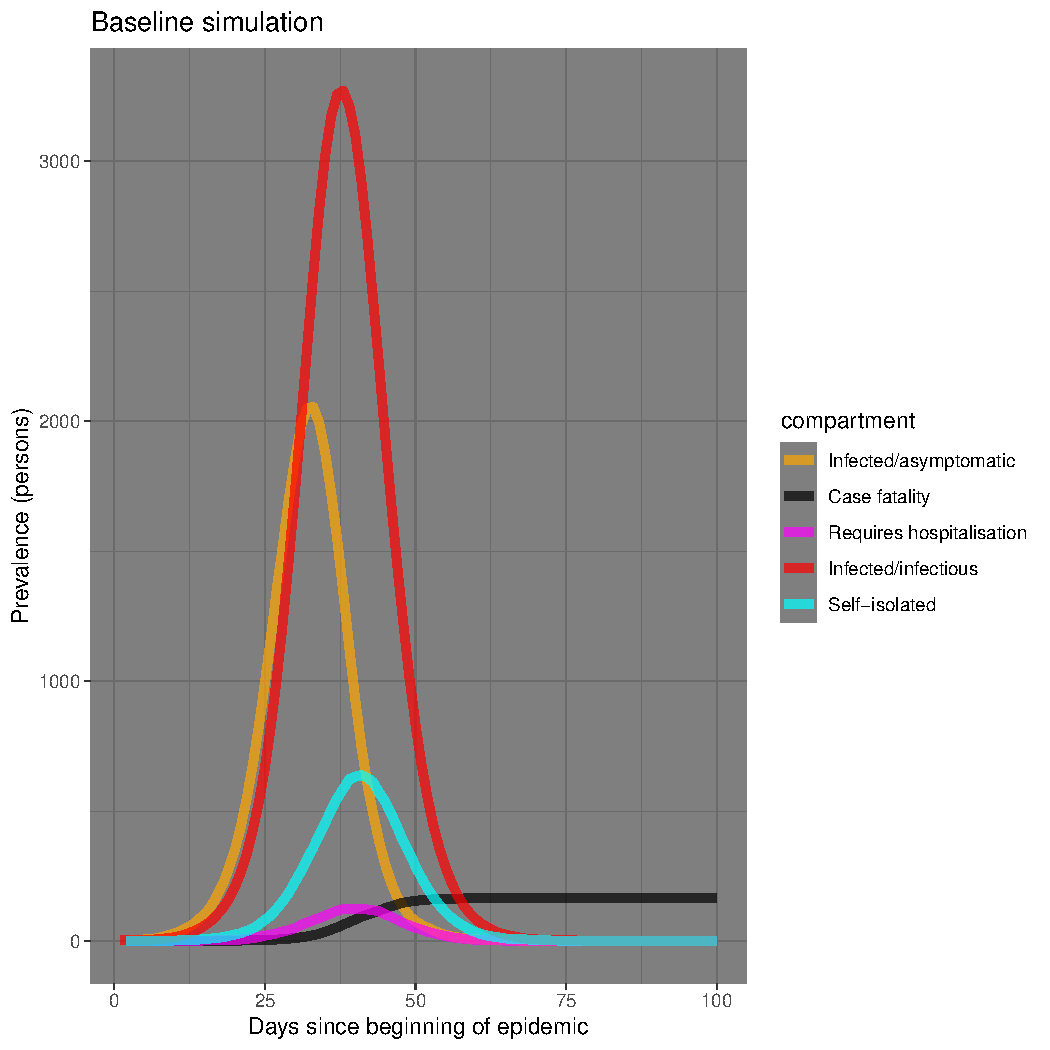
\includegraphics[width=\maxwidth]{figure/unnamed-chunk-25-1} 

\end{knitrout}

\begin{knitrout}
\definecolor{shadecolor}{rgb}{0.969, 0.969, 0.969}\color{fgcolor}\begin{kframe}
\begin{alltt}
\hlcom{# get the S-> E compartment flow, which is our daily}
\hlcom{# incidence rate}
\hlstd{incidence_counts} \hlkwb{<-} \hlstd{baseline_sim}\hlopt{$}\hlstd{df} \hlopt \hlkwd{select}\hlstd{(time, se.flow)}
\hlcom{# uncount them}
\hlstd{incident_case_dates} \hlkwb{<-} \hlstd{incidence_counts} \hlopt \hlkwd{uncount}\hlstd{(se.flow)} \hlopt
    \hlkwd{pull}\hlstd{(time)}
\hlcom{# convert to an incidence object}
\hlstd{incidence_all} \hlkwb{<-} \hlstd{incident_case_dates} \hlopt \hlkwd{incidence}\hlstd{(.)}

\hlcom{# plot the incidence curve}
\hlkwd{plot}\hlstd{(incidence_all)}
\end{alltt}
\end{kframe}
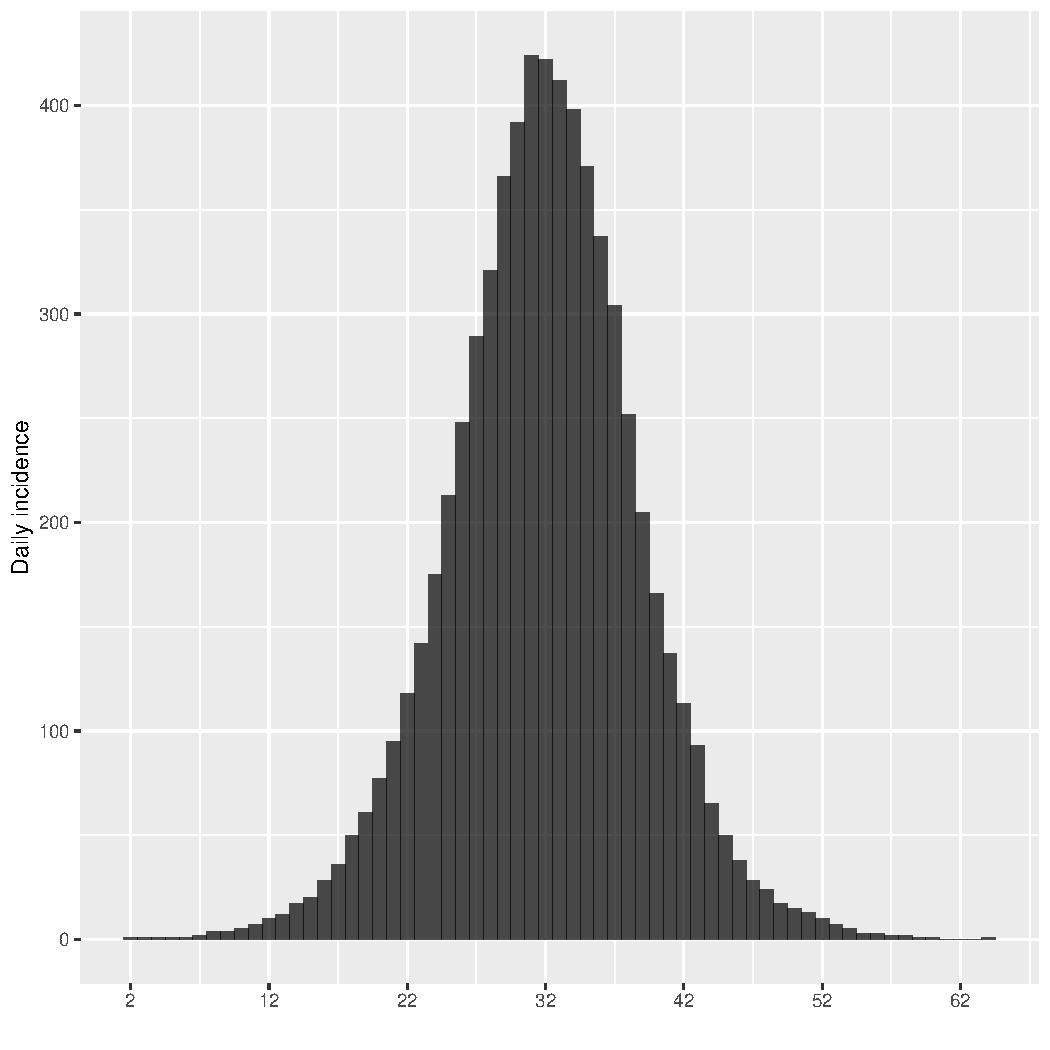
\includegraphics[width=\maxwidth]{figure/unnamed-chunk-26-1} 

\end{knitrout}

\begin{knitrout}
\definecolor{shadecolor}{rgb}{0.969, 0.969, 0.969}\color{fgcolor}\begin{kframe}
\begin{alltt}
\hlkwd{toc}\hlstd{()}
\end{alltt}
\begin{verbatim}
## Time to complete: 38.996 sec elapsed
\end{verbatim}
\end{kframe}
\end{knitrout}

\end{document}
